%% 美赛模板:正文部分
\newcommand{\upcite}[1]{\textsuperscript{\textsuperscript{\cite{#1}}}}
\documentclass[12pt]{article}  % 官方要求字号不小于 12 号,此处选择 12 号字体
\usepackage{enumitem}
\usepackage{threeparttable}
% 本模板不需要填写年份,以当前电脑时间自动生成
% 请在以下的方括号中填写队伍控制号
\usepackage[2314669]{easymcm}  % 载入 EasyMCM 模板文件
\problem{D}  % 请在此处填写题号
\usepackage{mathptmx}  % 这是 Times 字体,中规中矩 
\usepackage{setspace}
\usepackage{comment}

\usepackage{graphicx}  %插入图片的宏包
\usepackage{float}  %设置图片浮动位置的宏包
\usepackage{subfigure}  %插入多图时用子图显示的宏包

\usepackage[table,dvipsnames]{xcolor} 
\usepackage{amsmath}
%\usepackage{mathpazo}  % 这是 COMAP 官方杂志采用的更好看的 Palatino 字体,可替代以上的 mathptmx 宏包

\title{Determination of SDGs Priorities Based on Directed Network and Multi-Strategy Evaluation}  % 标题

% 如需要修改题头(默认为 MCM/ICM),请使用以下命令(此处修改为 MCM)
%\renewcommand{\contest}{MCM}

% 文档开始
\begin{document}

\numberwithin{figure}{section}%图表按章节编号

\numberwithin{table}{section}%图表按章节编号
\numberwithin{equation}{section}
% % 此处填写摘要内容
% \begin{abstract}
% The Sustainable Development Goals (SDGs) represent a universal set of goals that are interconnected in a complex network of interactions. Exploring the interlinkages between goals and establishing development priorities is essential for advancing the agenda of the United Nations. In this paper, we develop models to analyze the interlinkages between indicators of the goals, propose multiple strategies to assess the priorities of goals, and reveal the dynamic changes in network structure resulting from changes in indices.


% In \textsc{Task 1:} 
% First, we collect data from UNSD and select 117 representative indicators of the Goals under the UN IAEG-SDG standard. Then, the Strength of Interlinkage is computed to capture the possible causal relationship between nodes. To improve network performance, the threshold for the interlinkage is set at 0.6. Next, we take each indicator as a node and calculate the Strength of Interlinkage between indicators as weights to construct a directed Sustainable Development Goals Network.

% In \textsc{Task 2:} 
% We propose two strategies to determine the priorities of the 17 goals in the network: first, we calculate the network centrality of each node using degree centrality, closeness centrality, and betweenness centrality; then, the Network Influence is calculated to measure the prompt effects of an indicator on the entire network. Taking into account the transitivity of influence of network nodes, we introduced the concept of second-order network for improvement and calculated the priority ranking of the final 17 goals. We then clustered the network using community detection and found that Targets 7, 8, 9, 10, and 17 belonged to the same class; while Targets 1, 2, 3, 4, and 16 belonged to the same class. Finally, we predicted the implementation effect of priorities from the three dimensions of the Venn diagram: economy, society, and environment.


% In \textsc{Task 3: } 
% We select the No Poverty goal as the analysis object, remove the network nodes corresponding to all indicators under the target and the edges associated with them, obtaining the derived subgraph of the original network graph. We then calculate the centrality index and influence index of the sub-network, thus obtaining the new priority ranking of network nodes. The changes in the network priority ranking in the selected regions are in line with local conditions, verifying the rationality of the model.

% In \textsc{Task 4 \&  5:}
% We survey the literature to investigate the degree of alignment between the 17 sustainable development goals of the selected regions and their own development strategies, and establish the Consistency Index indicator to measure their consistency. Secondly, we adjust the consensus values for the indicators most impacted by COVID-19 and analyze the adjusted priorities. Finally, based on the three strategies established above, we extend the established model to the field of business management from the perspectives of network centrality, individual index influence, and organizational strategic consistency.


% \end{abstract}
\begin{abstract}The Sustainable Development Goals (SDGs) represent a universal set of goals that are interconnected in a complex network. Exploring the relationship between goals and determining development priorities is essential for advancing the agenda of the United Nations. In this paper, we develop models to analyze the interlinkages between indicators of the goals, propose \textbf{Multi-Strategy  Evaluation Model(MSE)} to assess the priorities of goals, and reveal the dynamic changes in network structure.

In \textsc{Task 1:} 
First, we employ the IAEG-SDG data in China and select 134 representative indicators. Then, the strength of interlinkage is computed using \textbf{Granger notion of causality } to capture the possible causal relationship between indicators. The threshold for the interlinkage is set to filter the weak  Strength of Interlinkage, making the structure of network clearer. In order to obtain the interconnection strength between each two goals, we calculate the total value of Strength of Interlinkage of each indicator. Finally, a directed network is created.

In \textsc{Task 2:} 
We propose two strategies to determine the priorities of the 17 goals: first, we calculate the \textbf{network centrality} of each indicator using eigenvector centrality, closeness centrality and betweenness centrality.  Second, considering the sum of influence of an indicator on the network and the transitivity of influence of network nodes, we introduce the concept of \textbf{second-order network}. Integrating the two strategies, we calculate  the priority rank of the 17 goals and conclude that we should prioritize Goal 8. We cluster the network using \textbf{community detection} and find that 17 SDGs are divided into three categories. If Goal 8 is prioritized, the economic goals represented by it will develop promptly in the next 10 years.


In \textsc{Task 3: } 
We select the Goal 1(No Poverty) as the analysis object, remove the network nodes and edges belonging to Goal 1, obtaining the derived sub-graph of the original network. We recalculate the centrality index and influence index of the sub-network and obtain the new priority ranking of goals, discovering that Goal 6(Clean Water and Sanitation) is prioritized. The changes of priority ranking in the selected regions are in line with local conditions, verifying the rationality of the model. Ultimately, Over Prosperity and Harmonious Coexistence Between People and Nature are proposed to the UN based on two perspectives.

In \textsc{Task 4 \&  5:}
In order to measure the impact of international events on our network, we define the \textbf{Consistency Index} to measure the consistency between the 17 SDGs of the selected region and its development strategies. Then, we adjust the consistency index of the goals that are impacted by COVID-19 and summarize that Good Health and Well-being is prioritized. Finally, based on the three strategies established above, we extend the established model to other fields from the perspectives of network centrality, influence index and  consistency index.

    \vspace{5pt}
    \noindent \textbf{Keywords}:
    MSE, Granger Notion of Causality, Network Centrality, Second-Order Network, Community Detection, Consistency Index.

\end{abstract}


\maketitle  % 生成 Summary Sheet
\tableofcontents  % 生成目录


% 正文开始
\section{Introduction}
\subsection{Problem Background}
The application of network structure in target strategic decision-making has seen a steady increase in recent years, owing to its ability to effectively capture the connections between goals and indicators, thus providing a comprehensive overview of the development requirements of the SDGs. Moreover, the application of network models and algorithms facilitates the identification of key nodes and links, which in turn can be used to formulate effective strategies for achieving the SDGs. Taking into account the complexity and interdependence of the goals, network structure provides a comprehensive basis for making informed decisions and developing effective strategies.


\subsection{Restatement of the Problem}
The United Nations (UN) Sustainable Development Goals (SDGs) represent a universal set of goals that are interconnected in a complex network of
interactions\upcite{1}. They provide a framework for governments, businesses, and individuals to work together towards a more equitable, prosperous, and sustainable future. Studies have revealed varying degrees of interconnectedness among each of the goals and targets, while some scholars believe that the sustainable development goals in the current format need a unified framework  to avoid ambiguous application of SDGs\upcite{2}. Additionally, many factors such as technological advances, global pandemics, have had serious consequences on the UN Sustainability Goals. In this problem, we need to accomplish the following objectives:

\begin{itemize}
    \item Create a comprehensive network of the relationships between the 17 SDGs.  Assign priority levels to each goal  based on its contribution to UN development, and predict the achievements in the next ten years based on the established prioroties.
    \item Once one of the SDGs is achieved, predict the structure of the established network and the updated priorities of the goals. Then analyze the new goals that could be proposed to the UN for inclusion.
    \item Examine how technological advances, global pandemics, climate change, regional wars, and other international crises influence your team's network and the selection of priorities. Determine the significant effects on the UN's progress from a network perspective.
    \item  Extract the general characteristics and laws of the established network model and extend it to the field of operation and management.
\end{itemize}

% \subsection{Literature Review}
% A network analysis is ideal for representing complex and multidimensional problems, and it has been
% used in similar cases like SDGs, transportation systems and financial markets\upcite{2}. 
% It can also be used to study communication networks, organizational structure, and other complex systems.  Then the proposed goals and targets can be 
% seen as a network, in which links among goals exist 
% through targets that explicitly refer to multiple goals\upcite{3}.
\subsection{Our work}
\begin{itemize}
    \item[*] We made sufficient preparations of the model: we extracted the desired indicators from the IAEG-SDG data; then calculated the strength of interlinkage between indicators, and used a threshold to filter out edges with low strength in order to construct a network.
    \item[*] We designed Multi Strategy Evaluation(MSE) for prioritization: we calculated three types of centrality, namely eigen centrality, betweenness centrality, and closeness centrality; and then computed the network influence of each node.
    \item[*] 
We employed a second-order network to further quantify the influence of indicators. This network could provide a more precise and comprehensive assessment of the network structure, thus enabling our model to better prioritize goals and indicators.
\item[*] 
We scored the priorities of the goals, and the goal with a high score was more likely to be given priority. Furthermore, we extended the ranking strategy of multi-objective network to the strategic decision-making field of organizations and enterprises.
\end{itemize}
\begin{figure}[htbp]
\centering
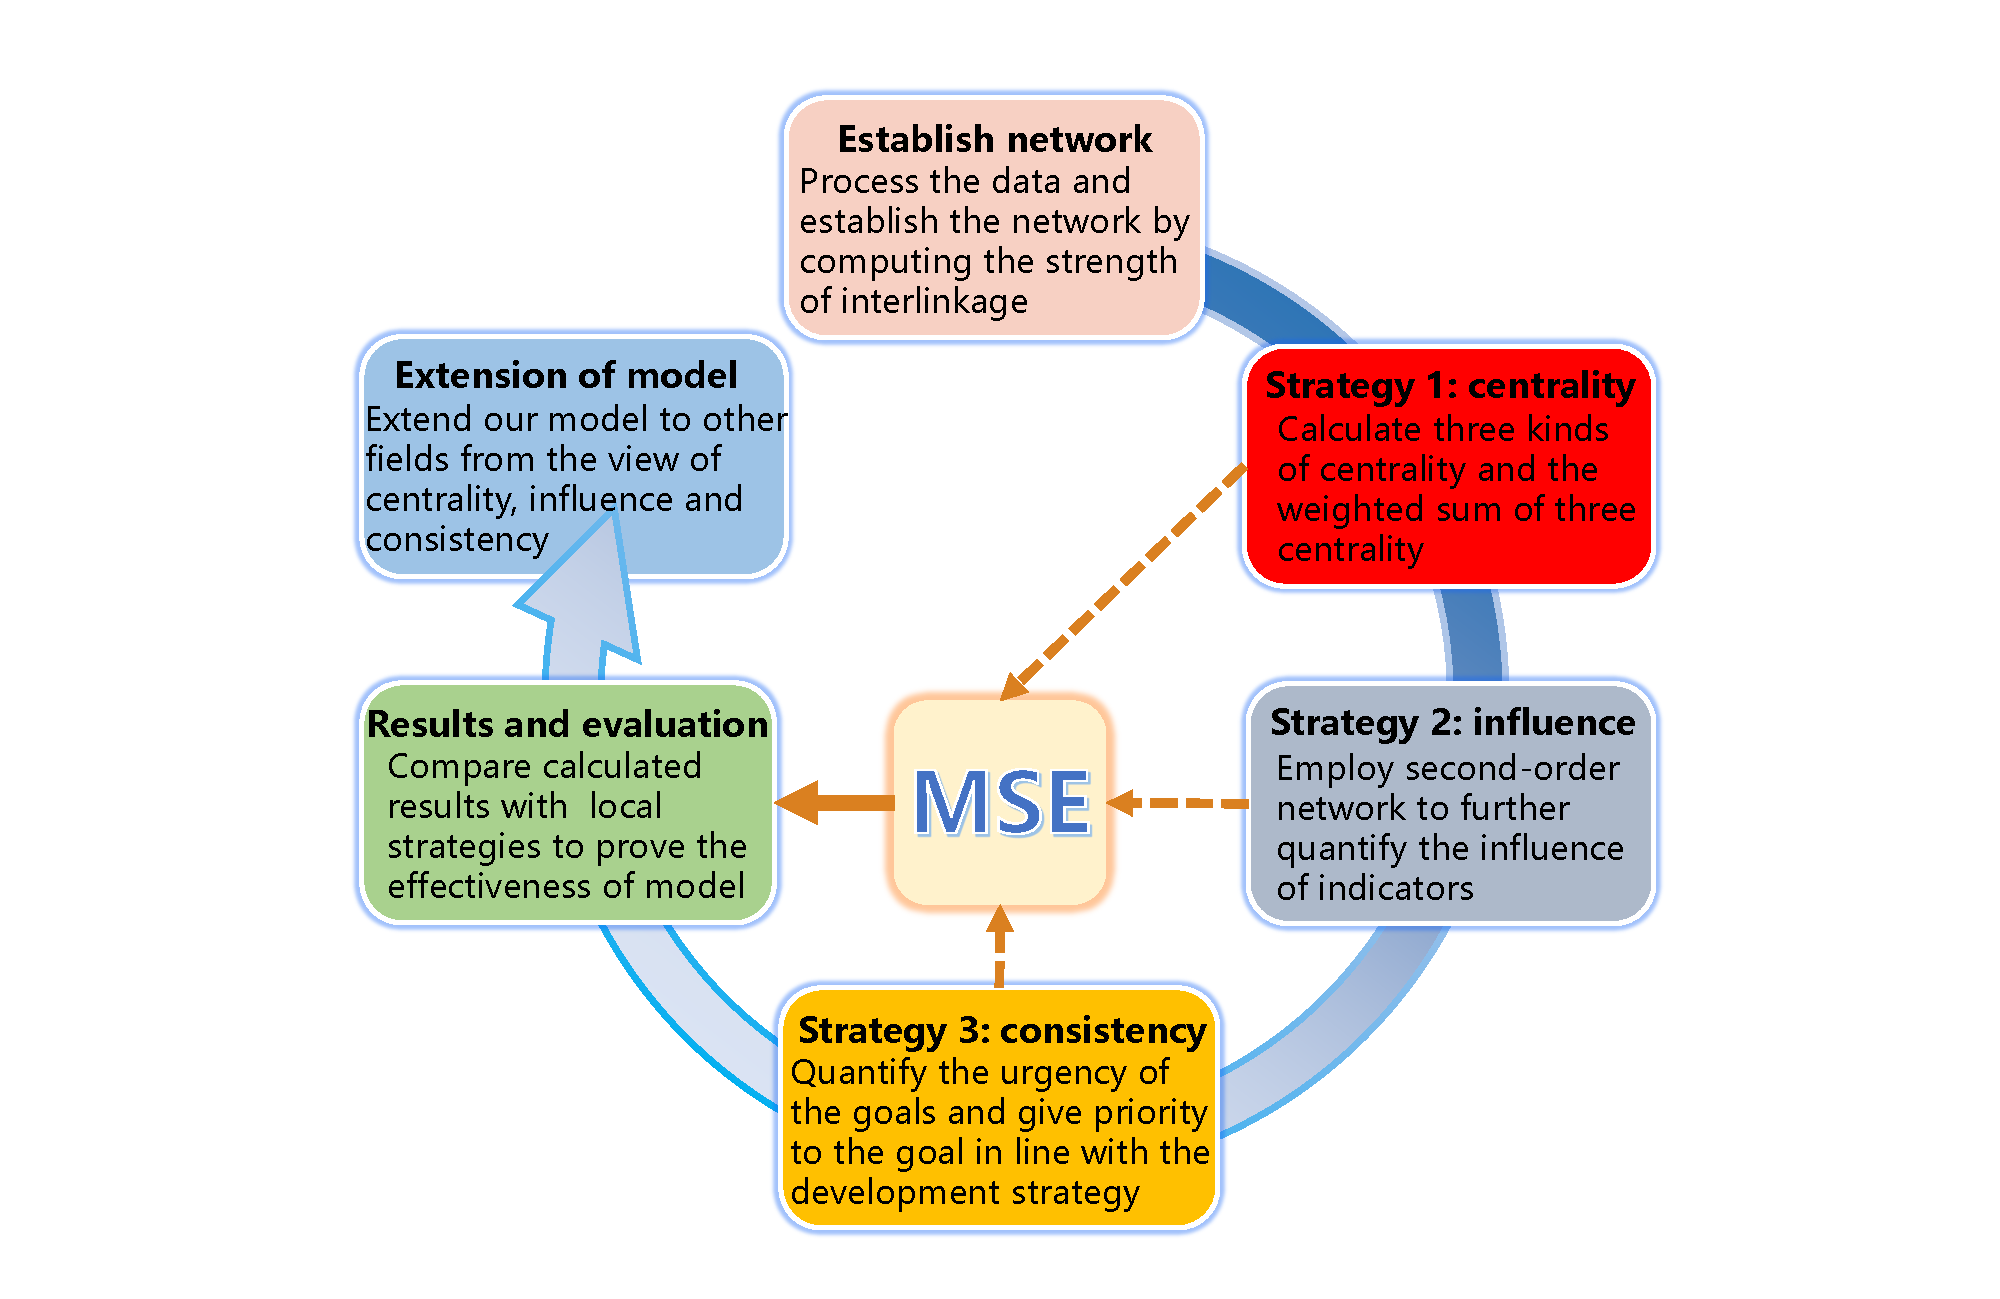
\includegraphics[width=.85\textwidth]{our work.pdf}
\caption{Our Work}\label{fig:result}
\end{figure}

\section{Preparation of the Models}
\subsection{Assumptions}
We made the following assumptions  in order to facilitate our modeling.  These assumptions laid the foundation for our subsequent analysis.

 $\bullet$ Assuming that the data is accurate and reliably sourced, which  means our analysis
accords with the truth.

 $\bullet$ Assuming that the sub-goals we have chosen are representative of the 169 strategies under the 17 Sustainable Development Goals (SDGs).

$\bullet$ Assuming that the weight between nodes in the network graph is directional, which means that the influence between two nodes is asymmetric.


 

 

\subsection{Notations}
The primary notations used in this paper are listed in Table \ref{tb:notation}.

% 三线表示例
\begin{table}[!htbp]
\vspace{-1.0em}\begin{center}\begin{threeparttable}
  
\renewcommand\arraystretch{1.2}

\caption{Notations}
\begin{tabular}{cl}
	\toprule
	\multicolumn{1}{m{3cm}}{\centering \textbf{\itshape{Symbol}}}
	&\multicolumn{1}{m{11cm}}{\centering \textbf{\itshape{Definition}}}\\
	\midrule
	$\rho_{ij}^{asym}$&asymmetric strength of interlinkage between variable $i$ and $j$\\
	$\hat{\rho}_{ij}^{asym}$&estimate of asymmetric strength of interlinkage between variable $i$ and $j$\\
 % $I_i^{1st}$&influence of indicator $i$ on its closest neighbours\\$I_i^{2nd}$&influence of indicator $i$ on its closest neighbours by a factor $0.5$
 % \\ 
 $I_i^{Total}$&total influence from indicator $i$ on the second order\\
	$EC_i$ &eigenvector centrality of node $i$\\
 $CC_i$&closeness centrality of node $i$\\
  $BC_i$&betweenness centrality of node $i$\\
  $E_i$&network influence of node $i$\\
  $CI_i$&consistency index of goal $i$\\
	\bottomrule
\end{tabular}\label{tb:notation}
\end{threeparttable}
\begin{tablenotes}
    \footnotesize
    \item[1] 
Symbols appearing in formulas but not in tables are explained in the text.
\end{tablenotes}
\end{center}\vspace{-1.0em}
\end{table}

\section{\textsc{Task 1:} Sustainable Development Goals Network Analysis Based on SNA}
\subsection{Model Overview}
According to Task 1, we need to use 17 goals and their related goals as nodes to establish a directed network connection graph to present the relationship between the goals. Firstly, we select 134 representative indicators as nodes of the network,  conducting  data processing. Then a 134-order cross-impact matrix is built  to calculate the weight of the edge between two nodes. By setting threshold to remove edges with less influence, we obtain the edges of the network, establishing the  Sustainable Development Goals Network.

\subsection{Data Processing}
To ensure accuracy in our model, in the first step, using the United Nations Statistics Division as the data source, we obtain scores for each country across 134 indicators of the 17 Sustainable Development Goals (SDGs). To avoid overfitting the model, we select the Tier 1 variables under the UN IAEG-SDG standard as network nodes. 

For some indicators (such as the proportion of the population below the poverty line), smaller is better, while for others (the proportion of the population with household access to basic services) larger is better, leading to ambiguity about the meaning of increasing indicator values. In order to resolve this issue, we process the data in the same direction; an increase in the indicator value implies that it is conducive to the realization of the SDGs. The data processing is shown in the Figure \ref{fig:result}. The selected  indicators under each Goal are shown in the appendix.


\begin{figure}[htbp]
\centering
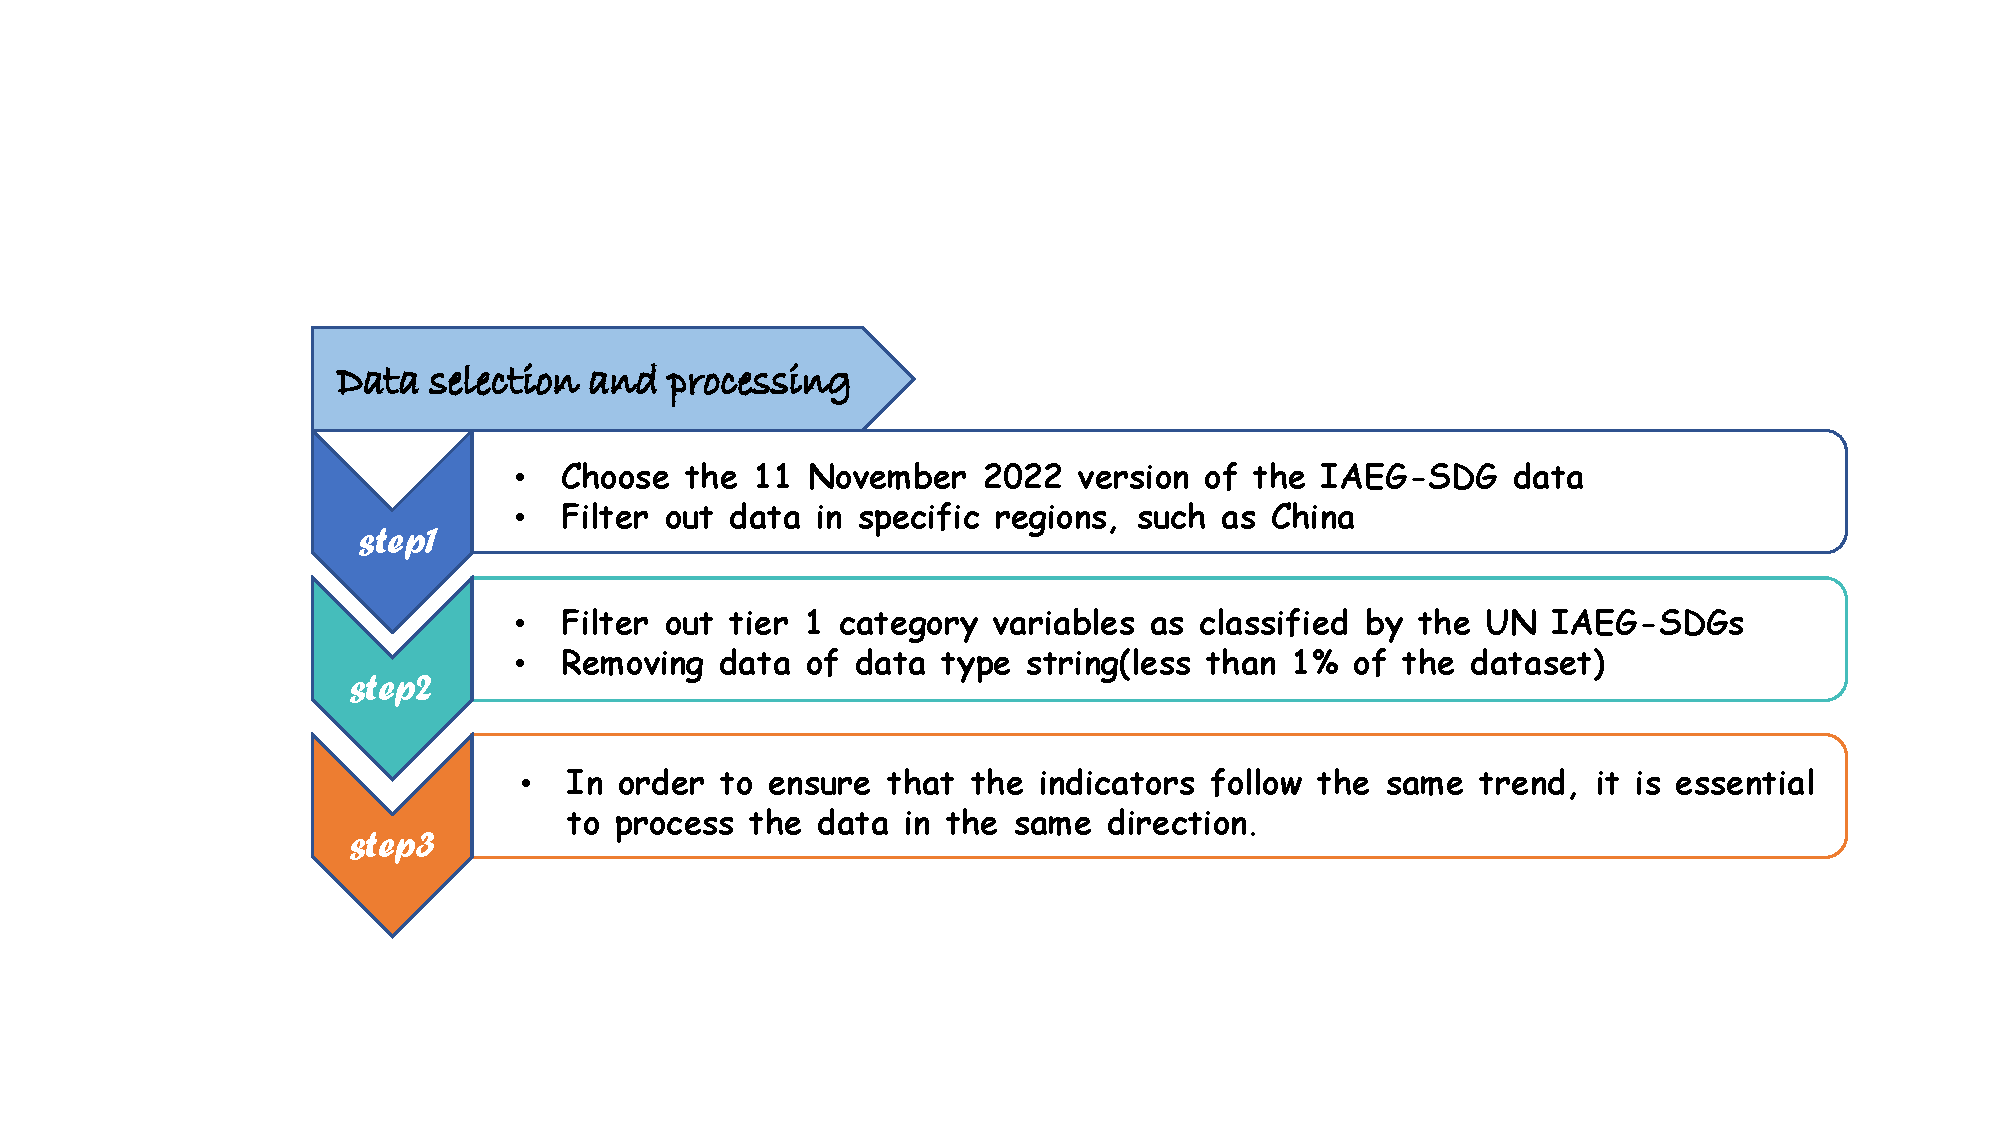
\includegraphics[width=.95\textwidth]{data_process.pdf}
\caption{Data Processing}\label{fig:result}
\end{figure}



\subsection{Sustainable Development Goals Network }

\vspace{0.7mm}\begin{itshape}
\textbf{$\blacktriangleright$ Selecting of Indicators of the SDGs}\end{itshape}


% \subsubsection{Selection of Indicators of the SDGs}
The seventeen goals of the SDGs are further divided into 134 indicators, which are then subdivided into individual indicators. Many studies focus on the hierarchy of the SDGs, clustering
the 17 goals under the three pillars of SD, linking every goal with a single pillar\upcite{3}. 

In order to facilitate the implementation of a global indicator framework, we used mostly Tier 1 categorical variables that were classified by the UN IAEG-SDG. These indicators are conceptually clear, with established international methodologies and standards, and are routinely produced by at least half of the population of each country or region that they relate to. Though Tier 1 indicators do not comprehensively cover all SDGs, they provide us with the most essential variables that are accepted by most CSOs across countries\upcite{2}.
% \subsubsection{Establishing of Strength of Interlinkage Matrix }

\vspace{0.7mm}\begin{itshape}
\textbf{$\blacktriangleright$ Establishing of Strength of Interlinkage Matrix }\end{itshape}

In a network topology, the edges between two nodes represent the degree of connection.  To capture the possible causal relationship between Node $i$ and $j$ in the network, we  use
the Granger notion of causality and define an asymmetric strength
of interlinkage as 
\begin{equation}
\rho _{ij}^{asym}=\left( E\left[ i_{lag}j \right] -E\left[ i_{lag} \right] E\left[ j \right] \right) /\sqrt{\left( E\left[ i_{lag}^{2} \right] -E\left[ i_{lag} \right] ^2 \right) E\left( j^2-E\left[ j \right] ^2 \right)},
\label{eq:3.1}
\end{equation}
where $i_{lag}$ and $j_{lag}$ are time-lagged versions of $i$ and $j$\upcite{1}.

 In our application, $i$ and $j$ are two different indicators for the SDGs, e.g., ''Proportion of population in a country below the international poverty line", and ''Total unemployment rate".
 Note that if we assume stationarity conditions on the viables, $E[i_{lag}]=E[i],E[i_{lag}^2]=E[i^2]$ hold\upcite{1,5}.  Since  $i$ and $j$ are
timeseries data, and are also available for different regions, we estimate  the asymmetric strength of interlinkage that
captures a Granger notion of causality by
\begin{equation}
\hat{\rho}_{ij}=\frac{1}{sd_isd_j}\frac{1}{N}\frac{1}{T-2}\sum_{k=1}^N{\sum_{k=2}^T{\left( i_k\left( t-1 \right) -\bar{i}_k \right) \left( j_k\left( t \right) -\bar{j}_k \right)}},
\label{eq:3.2}
\end{equation}
where the $\bar{i}_k$ and $\bar{j}_k$ represent the time-average of our selected region's $i$ and $j$, and $sd_{i}$, $sd_j$ represent the standard deviation of variables $i$ and $j$ respectively\upcite{1}. With $\rho_{ij}^{asym}$ as the element in row $i$ and column $j$, a weight matrix $A=(\rho_{ij}^{asym})_{N\times N}$ can be established, where $N$ represents the number of elements in the matrix, i.e., the quantity of nodes in the network.
% 以$\rho$为第i行第j列的元素,可以建立起邻接矩阵$A=(\pho _ij)_{N\times N}$,其中N代表矩阵中元素的数量,即网络的节点数量。


\vspace{0.7mm}\begin{itshape}
\textbf{$\blacktriangleright$ Selecting Representative Region}\end{itshape}



% \subsubsection{Selection of Representative Region}
% The SDGs have varying emphases in different regions, necessitating the selection of representative regions for effective benchmarking and the identification of the need for different dynamics of working within the SDGs.
Given the highly contextual nature of the effects of goals on one another, it is essential to consider the specific context when assessing them\upcite{11}. This is in line with previous research\upcite{12} which highlighted the importance of interpreting the goals with respect to the current status and trends of the issues raised by the indicators, the available resources and policy efforts, and the objectives of the 2030 Agenda. Each government is expected to set its own goals based on the national context (UN 2015).

To ensure our analysis is regionally reflective, we selected sample data from China, owing to the chanllenges it faces on SDGs\upcite{4,5}.
% The degree to which China's SDGs are implemented directly impacts the attainment of global Sustainable Development Goals.
After a comprehensive examination of China's sustainable development agenda, the network model can be extended to other regions, including Southeast Asia, Japan, and the United States.



%% 在网络拓扑结构中,每两个节点之间的边代表节点间的关联程度

\vspace{0.7mm}\begin{itshape}
\textbf{$\blacktriangleright$ Constructing  Sustainable Development Goals Network }\end{itshape}

% \subsubsection{Constructing  Sustainable Development Goals Network }

In the Strength of Interlinkage Matrix, the element $\rho_{ij}^{asym}$ denotes the weight of the edge between node $i$ and node $j$, thus forming a directed complete simple graph. If the weight of the edge between two nodes is too small, it can be assumed that the correlation represented by the edge does not exist. 
When different thresholds $\sigma$ are chosen, the network topology will be altered. The most conspicuous performance is the number of edges and points. Table \ref{tab:3.1}  shows the number of network nodes and edges at different thresholds.
\begin{table}[h]\vspace{-1.0em}
\centering \caption{Number of Network Nodes and Edges at Different Thresholds.}
\begin{tabular}{c|c|c|c|c}
\hline\hline
          & $\sigma=0.2$ & $\sigma=0.4$ & $\sigma=0.6$ & $\sigma=0.8$ \\ \hline\hline
number of nodes & 134 & 134 & 134 & 134\\ \hline
number of edges & 5399 & 3699 & 2160 & 797 \\ \hline\hline
\end{tabular}\vspace{-1.0em}\label{tab:3.1}
\end{table}

To facilitate the subsequent normative analysis and improve network performance, we select $\sigma=0.8$ as the threshold of network edge weight, and edges greater than this threshold are considered to be valid and effective\upcite{6}. In the following analysis of Section 8, we adjust the threshold and analyze the alterations in network structure and performance brought about by varying thresholds.
\subsection{Analysis of the Results}

In the network constructed with indicators as nodes, there are 134 nodes and 797 edges in total. The presence of multiple overlapping relationships between edges hindered the intuitive display of the network topology. 

We calculate the total value of  Strength of Interlinkage of all indicators connected between each two goals under the 17 goals to obtain the interconnection strength between each two goals nodes, as presented in Figure \ref{fig:3.2}.


As shown in Figure \ref{fig:3.2}, the numerical numbers of the nodes correspond to their goal numbers; the direction of the arrow indicates the direction of influence; the color of the nodes indicates the category to which the goal belongs (red represents ecology, blue represents society, and green represents economy). Nodes of the same color belong to the same category; the thickness of an edge indicates the strength of influence between two objects.

\begin{figure}[htbp]
\centering
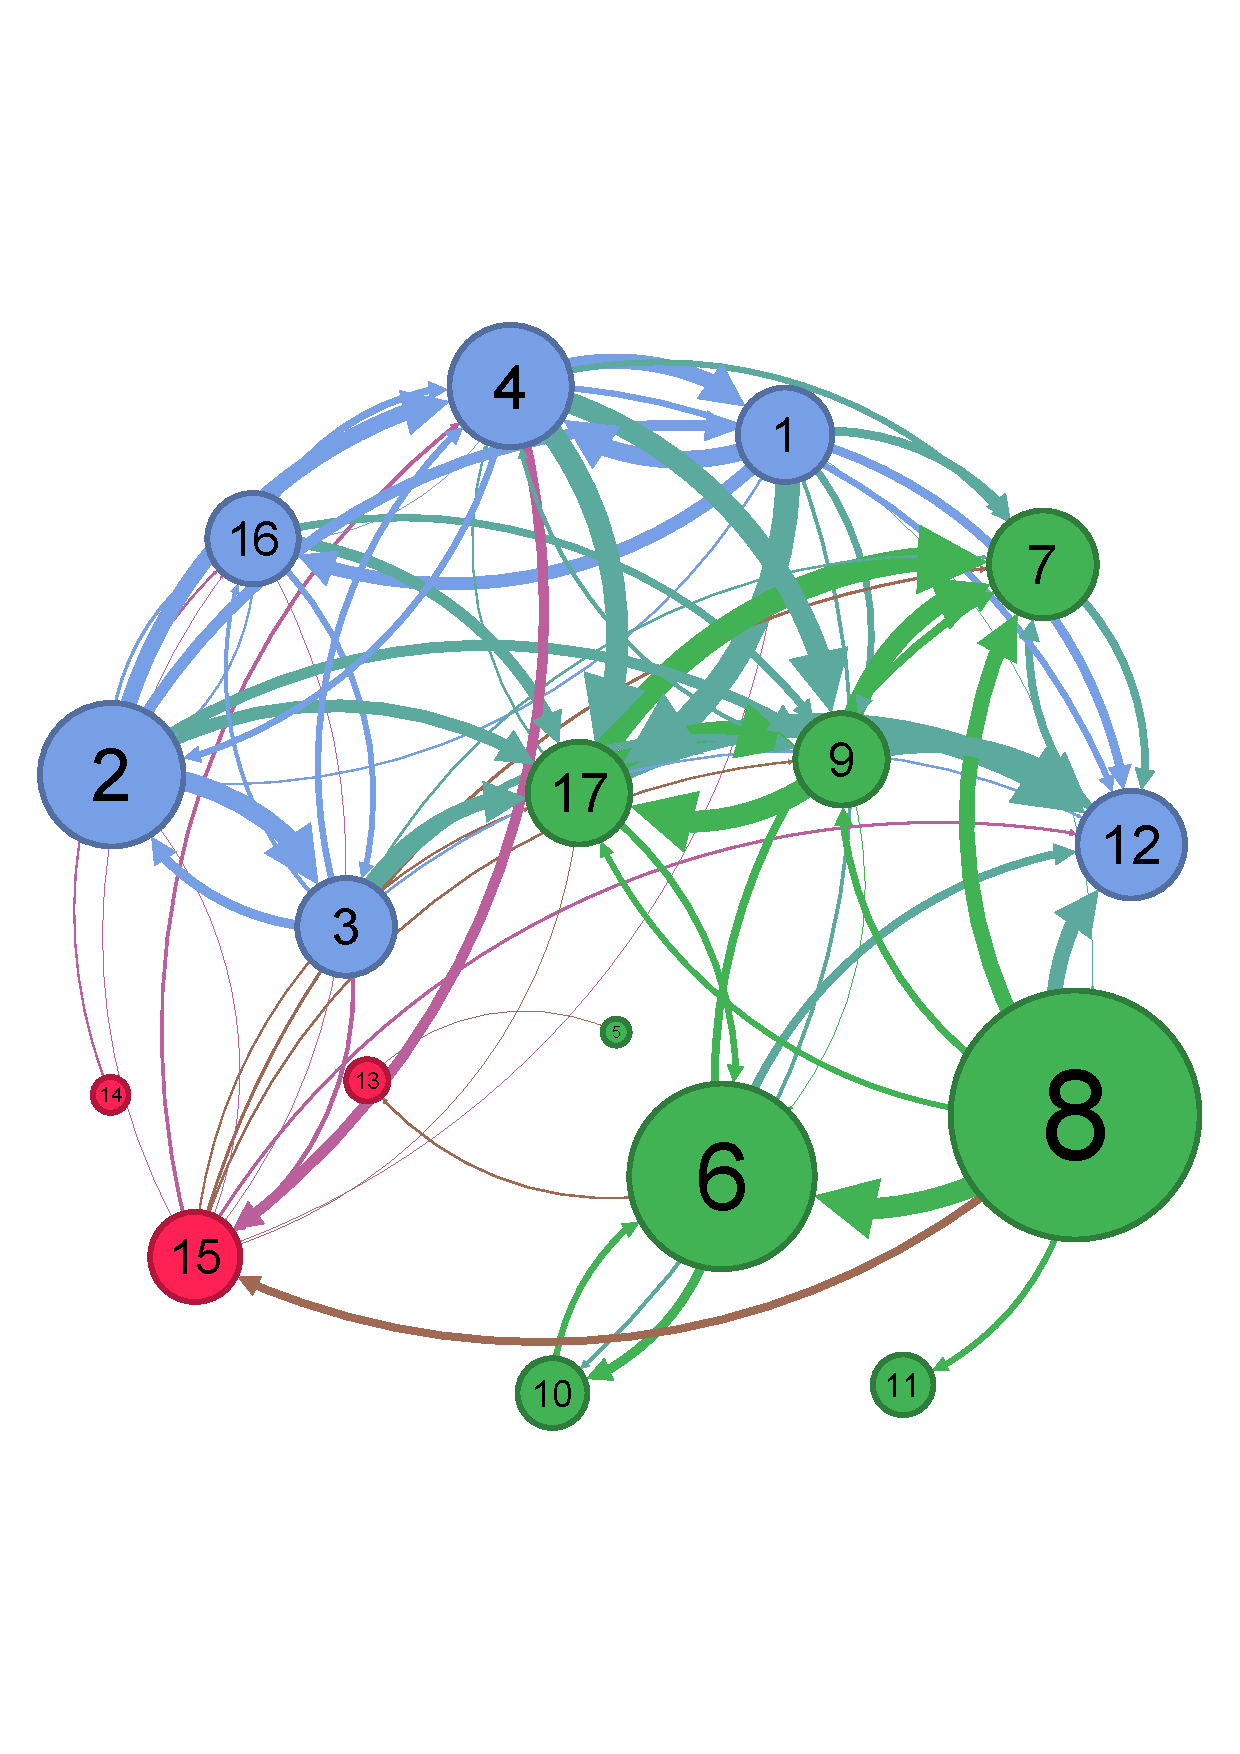
\includegraphics[width=.5\textwidth]{17goal.pdf}
\caption{Sustainable Development Goals Network }\label{fig:3.2}
\end{figure}
As evidenced by Figure \ref{fig:3.2}, there are more associations between goals of the same type, thus resulting in thicker lines between them. For example, among the blue nodes, the connection between nodes 2, 4, and 16 is thicker. This confirms the effectiveness of the network model we built, as it is consistent with the actual facts.
\section{\textsc{Task 2:} Dual-Strategy Sustainable Development Goals Network}

\subsection{Model Overview}
In \textsc{Task 1}, 
We construct a Sustainable Development Goals Network to study the correlations between the 17 goals. In order to establish the priority order of the 17  nodes, in the first step we introduce the centrality of network nodes as the first strategy to measure the importance of nodes.
% then measure the consistency between the existing strategy of the selected region (China) and the goals of SDGs as the second strategy, and 
Then we calculate the Network Influence  of each  indicator $i$, establishing the  Dual-Strategy Sustainable Development Goals Network. 
In order to account for the impact of the second-order network, we then revise and optimize the Dual-Strategy Sustainable Development Goals Network  and introduce the Total Influence Indicator. 
\subsection{Dual-Strategy Sustainable Development Goals Network}
\subsubsection{Strategy One: Calculation of Network Centrality}

Given the heterogeneous nature of complex networks, it is anticipated that the importance of nodes can be quantified by the network centrality, as the most central nodes are expected to be the most influential and can more efficiently disseminate their data than other nodes.
In order to evaluate the centrality of nodes from various perspectives, we choose three indicators: eigenvector centrality, closeness centrality, and betweenness centrality.

\vspace{0.7mm}\begin{itshape}
\textbf{$\blacktriangleright$ Eigenvector Centrality}\end{itshape}

A node in a network can be considered important if other important nodes follow it\upcite{6}.
Thus the importance of node $i$ can be defined by
\begin{equation}
    EC_i=x_i=c\Sigma_{j=1}^{n}a_{ij}x_j,
\end{equation}where $c$ is a constant of proportionality. Let  $ x=[x_1,\cdots,x_N]$, when the steady state is reached after several iterations, it can be written in the following matrix \begin{equation}
   x=cAx,
\end{equation}where x represents the characteristic variable corresponding to the eigenvalue $c^{-1}$ of matrix $A$. The entries of $x$ are called eigenvector centrality\upcite{6}. An indicator with higher eigenvector centrality is more likely to be connected to important indicators of the network.

\vspace{0.7mm}\begin{itshape}
\textbf{$\blacktriangleright$ Closeness Centrality}
\end{itshape}

Closeness centrality is determined by the average distance of each node to all other nodes.  It has the advantage to be very intuitive
and suitable to characterize a process where the information travel through the
shortest distances. Mathematically,
the closeness centrality of node $i$ is defined as
\begin{equation}
    CC_i=\frac{N}{\Sigma_{j=1,j\ne i}^N d_{ij}},
\end{equation}
where $d_{ij}$ is the length of the shortest path between node $i$ and $j$,  and $N$ is the number of nodes in the network\upcite{6}.   A node with high closeness centrality is typically closer to all other nodes of the network than a node with low closeness centrality, on average.



\vspace{0.7mm}\begin{itshape}
\textbf{$\blacktriangleright$ Betweenness Centrality}\end{itshape}

The betweenness centrality based on random walks is expressed as the expected number of visits to each node i during a random walk
\begin{equation}
BC_i=\Sigma^N_{a=1}\Sigma_{b=1}^Nw(a,i,b),
\end{equation}
where $w(a, i, b)$ is the number of times that $i$ is visited when a random walk of
length $n$ is performed from nodes $a$ to $b$\upcite{6}. An indicator with the highest betweenness centrality tend to have the most control over the information flow of the network, since it tends to be positioned between many other indicators.

% \subsubsection{Strategy Two: Assessing Alignment of SDGs with Society}
% Owing to the region and the resources available, the seventeen goals of the SDGs have different levels of implementation in China. 
% This paper evaluates the actual realization and implementation of each Sustainable Development Goals, dividing them into four categories. Then the assessment is then mapped to a numerical value via a simple additive scoring method\upcite{7}.


% Through evaluating China's performance on the seventeen interdependent goals, we can assess the effectiveness of the SDG implementation and determine the priority of the nodes.  
% Green, yellow, orange, and red signify the difficulty in achieving the corresponding Sustainable Development Goals (SDGs) in China, with green indicating the lowest difficulty and red indicating the highest, which is shown in Table \ref{tab:4.1}.
% \begin{center}
% \begin{table}[!htbp]\centering\caption{China's Performance on the SDGs}\label{tab:4.1}\begin{threeparttable}
% \begin{tabular}{ccccccccc}
% \hline
% \textbf{SDG1} & \textbf{SDG2} & \textbf{SDG3} & \textbf{SDG4} & \textbf{SDG5} & \textbf{SDG6} & \textbf{SDG7} & \textbf{SDG8} & \textbf{SDG9} \\ 
% % \midrule
% % \specialrule{0em}{1.5pt}{1.5pt}
% \hline
% \cellcolor{Yellow} Y & \cellcolor{BurntOrange} O &\cellcolor{BurntOrange} O &\cellcolor{LimeGreen} G & \cellcolor{BurntOrange} O & \cellcolor{BurntOrange} O &\cellcolor{BurntOrange} O &\cellcolor{LimeGreen}  G & \cellcolor{BurntOrange}O \\ \hline
% \textbf{SDG10} & \textbf{SDG11} & \textbf{SDG12} & \textbf{SDG13} & \textbf{SDG14} & \textbf{SDG15} & \textbf{SDG16} & \textbf{SDG17} & \\ \hline
% % \specialrule{0em}{1.5pt}{1.5pt}
% % \midrule
% \cellcolor{Red} R & \cellcolor{BurntOrange} O & \cellcolor{BurntOrange} O &
% \cellcolor{Red} R &
% \cellcolor{Red} R & \cellcolor{BurntOrange} O &
% \cellcolor{Red} R & \cellcolor{BurntOrange} O & \\ \hline
% \end{tabular}

% \end{threeparttable}\begin{tablenotes}
% \footnotesize
% \item[1] G(reen): SDG Achievement; Y(ellow): challenges remain; O(range) Significant challenges remain; R(ed) major challenges\upcite{7}.
% \end{tablenotes}
% \end{table}\end{center}

% To quantify China’s performance on the 17 goals for prioritizing network nodes, we map G, R, O, and R to $0$-$1$ to develop a Consistency Index $CI_i$. 
% Assuming China's performance efficiency in the $i$-th goal is $Goal_i$, and its discretization values are G, R, Y, O.
% Let the selected indicator be $a_i$, and the set of all indicators included in Goal $i$ be $Goal_i$. Then the indicator $a_i$'s  Consistency Index   $CI_i$ is given by the following:
% \begin{equation*}CI_i=
% \begin{cases}0.25,\quad &i\in Goal_j\& Goal_j=G,\\0.5,\quad &i\in Goal_j\&Goal_j=Y,\\0.75,\quad &i \in Goal_j\&Goal_j=O,\\1,\quad &i \in Goal_j\&Goal_j=R.
% \end{cases}
% \end{equation*}

\subsubsection{Strategy Two: Computing of the Network Influence of Node}

% If an indicator reinforces another indicator which has strong positive connections, its systemic impact can be highly significant. Conversely, if the other indicator has few weak positive connections, the positive effect will quickly dissipate and have little systemic impact\upcite{8}.

An indicator with a high row-sum can be regarded as a synergistic one that enhances the effect of prompts on the overall efficiency of the network.

Let $i \,R \,j$ denote the relation that there exists a directed edge from node $i$ to node $j$ in the network.
Let $E_i$, $E_j$ represents the network influence  of indicator $i$ and $j$ respectively, which are calculated by the following equation
\begin{equation}
    E_i=\Sigma_{j\in \{k|\,\,iRk\,\,\}}\rho_{ij}^{asym}.
\end{equation}

% \subsubsection{Dual-Strategies Intergration}
The interrelated nature of the SDG indicators implies that progress towards one indicator is also connected to other indicators through complex feedbacks\upcite{9}. 
In the Dual-Strategy Sustainable Development Goals Network, the two strategies focus on network centrality, policy consistency, and the second-order structure of the network, emphasizing the implementation of SDG strategies in specific regions.


A weighted linear average is utilized to combine strategies. For each strategy, the 
corresponding scores are normalized to the same scale (0–1) through the formula\upcite{8}:
\begin{equation}
    S_i=(S_t-\min(S))/(\max (S)-\min (S)),
\end{equation}
where $S_n$ is the normalized score of an indicator for a particular strategy, $S_t$ denotes the original score of an indicator for a particular strategy.

When it comes to weights for the two strategies, decision makers tend to attach different levels of importance to different Goals\upcite{9}. The final scores are calculated by the following equation
\begin{equation}
    S_{Final}=((S_{c1}\times W_{c1})+(S_{c2}\times W_{c2}))\times 100,
\end{equation}
where $S_{Final}$ is each indicator's final score, $S_{ci}$ represents the normalized score for  each indicator under strategy $i$\upcite{9}. 

\subsection{Modified Dual-Strategy Sustainable Development Goals Network}
% \subsubsection{Introduction of Second-Order Network}

\vspace{0.7mm}\begin{itshape}
\textbf{$\blacktriangleright$ Introduction of Second-Order Network}\end{itshape}

When analyzing the influence of a node on other nodes, we only considered the interaction between a selected indicator and its direct "adjacent" indicators, while disregarding how the adjacent indicator interacts with other indicators in turn. This means we only consider first-order interactions, thus failing to identify which indicators should be prioritized to maximize the performance of the entire network.


For example, the  indicator $2.1.1$ has a greater influence on  indicator $1.1.1$, that is, the  indicator $2.1.1$ can effectively promote the  indicator $1.1.1$, but indicator $1.1.1$ in turn has a greater negative impact on  indicator $10.7.3$, $12.c.1$ and $13.2.2$. The progression of indicators with greater influence will make the implementation of other indicators more difficult\upcite{8}. 

Consequently, prioritizing indicator $i$ may be a counterproductive strategy if we consider the broader impact on the network. To avoid the problem, decision makers need to consider not only a section of interactions but also deeper interactions when prioritizing, that is, we need to comprehend its effect on the overall system network performance\upcite{8}.

% \subsubsection{Consider the Priority order of Second-Order Networks}

\vspace{0.7mm}\begin{itshape}
\textbf{$\blacktriangleright$ Consider the Priority order of Second-Order Networks}\end{itshape}


In order to generate information that can guide prioritization, vigilance is needed to avoid factors that cause a negative impact; we need to consider how the impact of an action propagates in the network. If one metric reinforces another metric that has a strong positive relationship with the others, then the impact of the original metric on the overall system is significant. Conversely, if the positive link for another indicator is small or weak, the positive effect dissipates quickly without much systemic impact. Even more, a situation where another indicator in turn has a large negative impact on other indicators, thus creating a detrimental systemic effect, should be avoided.
A negative connection to a indicator that in turn has strong positive connections may be a reason for caution as negative impact can spread.


To test the hypothesis that the priority of indicators would change if second-order effects were taken into account, we calculate the total impact of our chosen indicators on the second-order network. This includes the influence of the neighboring indicators' neighbors. Figure \ref{fig:4.1} illustrates the concept of transitioning from considering only first-order interactions to second-order interactions.

\begin{figure}[htbp]
\centering
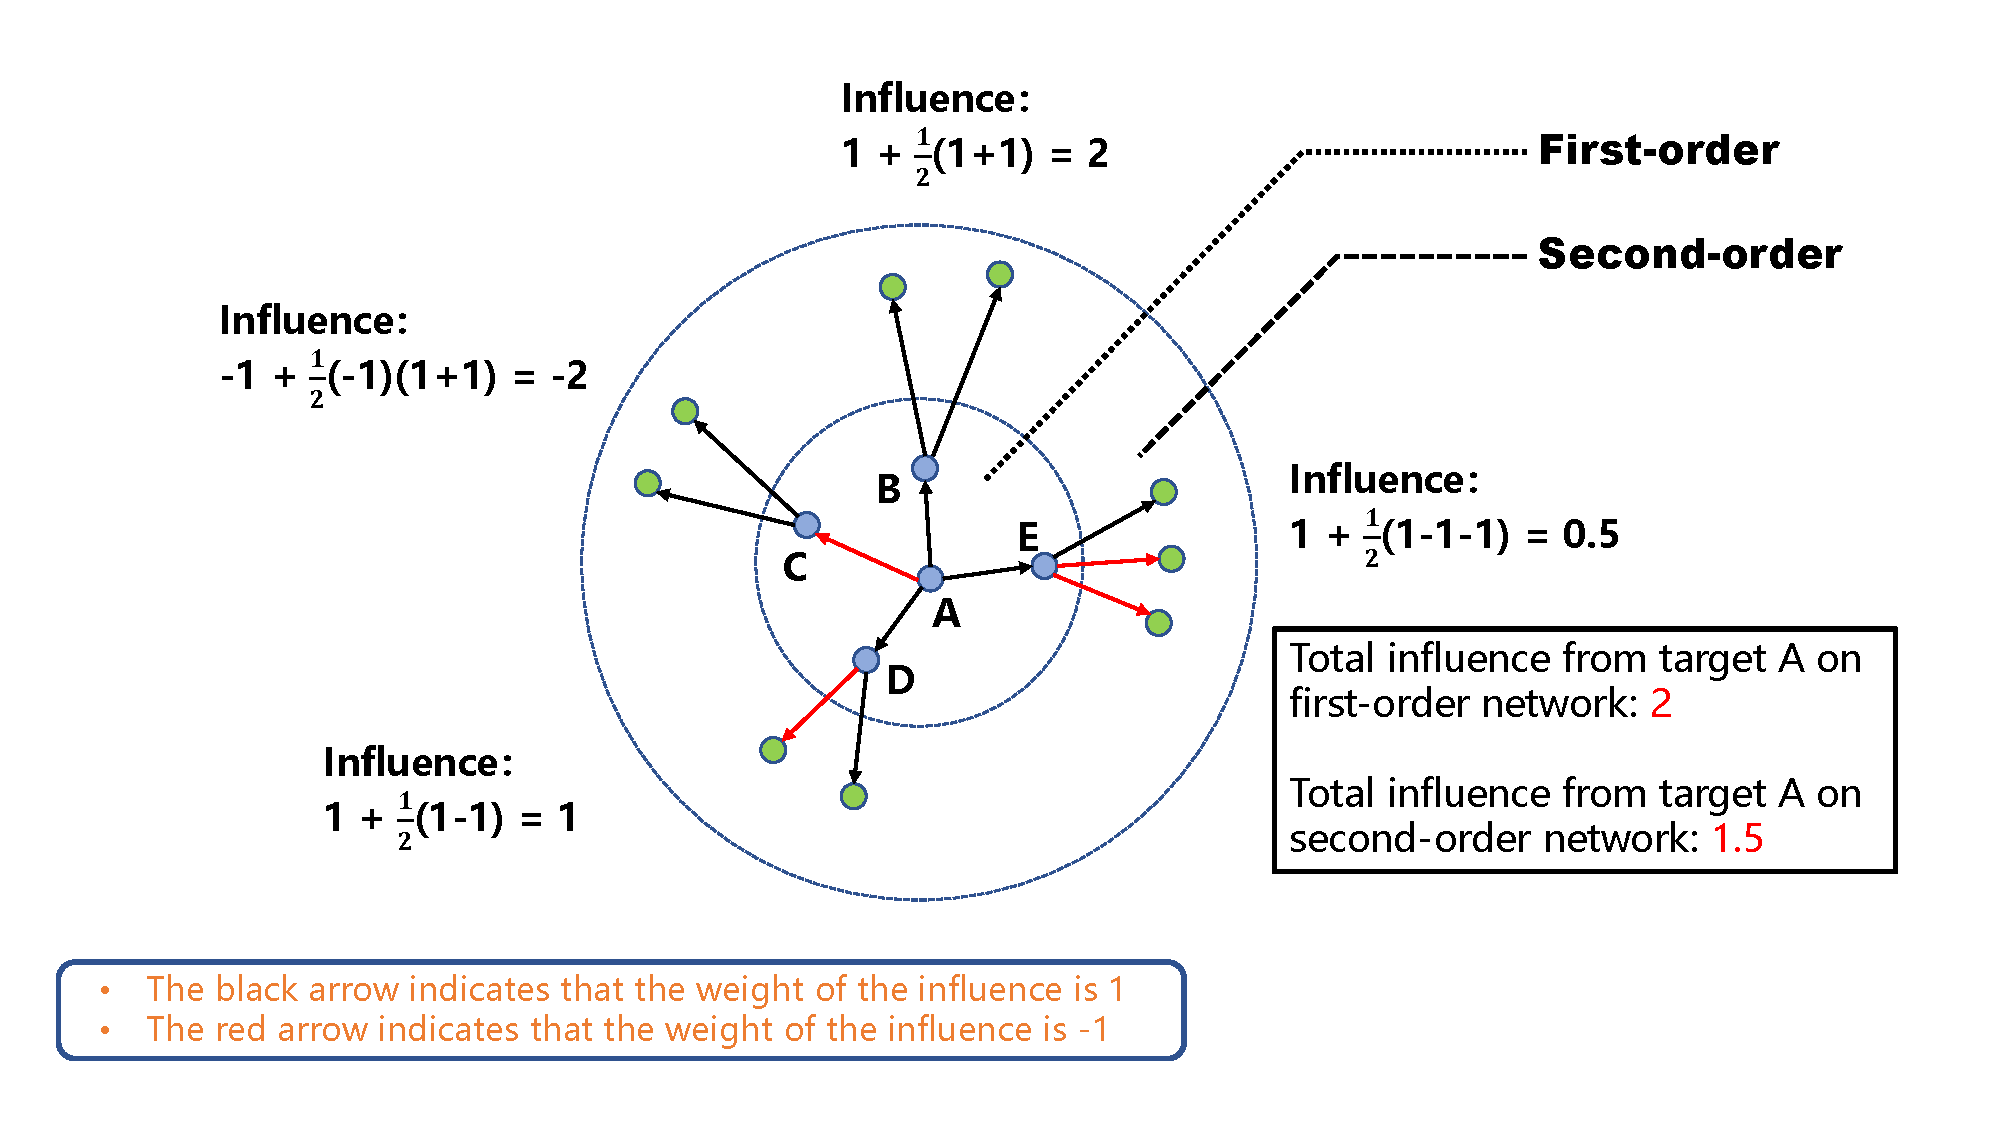
\includegraphics[width=.85\textwidth]{second-order.pdf}
\caption{Conceptual Figure Showing the Total Influence  When Considering  Second-order Interactions
}\label{fig:4.1}\vspace{-1.0em}
\end{figure}

%%%%%%%%%%%%%%%%%%%%%%%%%%%%%%%%%%%%%%%%%%%%%%%%%%%%%%%%%%%%%%%%%%%%%%%%%%%%%%%%%%%%%%%%%%%%%%%%%%%%%%

It shows how the total impact of the indicator on the network changes when second-order interactions are included in the evaluation. According to Figure \ref{fig:4.1} positive links in the second layer do not necessarily counteract the negative links in the first layer; on the contrary, the negative influence will create ripples and spread throughout the network.
\begin{comment}
为了生成可以指导确定优先级的信息,需要提高警惕以避免造成负面影响的因素,我们需要考虑一个行为造成的影响如何在网络中蔓延。如果一个指标强化了另一个指标,而另一个指标又与其他指标有着强烈的正向联系,那么原始指标对整个系统的影响是非常显著的。然而,如果另一个指标的正向联系很少或很弱,那么积极效应很快就会消失,不会产生太多的系统性影响。甚至,另一个指标反过来又对其他指标产生大量负面影响,从而产生负面的系统影响,这种情况是需要避免的。同样的,A negative connection to a target that in turn has strong positive connections may be a reason for caution as negative impact can spread.(这句很好 我直接粘英文)。
为了验证如果考虑到二阶效应,指标的优先级将会改变的假设,我们计算了我们选择的指标对二阶网络的总影响。也就是说,我们包括了邻近指标的邻居(neighbouring indicator’s neighbour)的影响。图7显示了从只考虑一阶交互到二阶交互的概念思想【这里可以画个示意图到时候】它显示了如果我们在评估中包括二阶相互作用,指标对网络产生的总影响是如何变化的。图7强调了第二层中的正链接并不一定能抵消第一层中的负链接,相反,负影响会在网络中产生涟漪并扩散。
\end{comment}

We define the total influence metric to measure the second-order effect, which is calculated by
\begin{equation}
    I_i^{Total}=I_i^{1st}+\frac{1}{2}\Sigma I^{2nd}=E_i+\frac{1}{2}\Sigma_{j\ne i}\rho_{ij}^{asym}E_j,
\end{equation}
where    $I_i^{1st}$ represents the influence of indicator $i$ on its closest neighbours, $I_i^{2nd}$ is the influence from $i$'s neighbour's on their neighbours weighted by a factor $1/2$\upcite{8}, $\rho_{ij}^{asym}$ denotes the strengths of interlinkage from node $i$ to node $j$ as defined in (\ref{eq:3.1}).


\subsection{Analysis of the Results}
\subsubsection{Analysis of the Prioritiazation}

\vspace{0.7mm}\begin{itshape}
\textbf{$\blacktriangleright$ Strategy One: Network Centrality}
\end{itshape}


The Network centrality of an indicator in a network measures the relative significance  of its corresponding node within a network.
In the established Strength of Interlinkage Matrix, the column-sum indicates the total influence of an indicator on the other indicators, while a high row-sum suggests that an indicator has a large net positive impact on the other indicators\upcite{8}. 


% However, the row-sum does not indicate whether the influence consists of a large number of weak influence on many indicators or a few strong ones, nor the distribution between positive and negative interlinkages.
% Table \ref{tab:4.2} shows the top two and bottom two values of the row-sum, and lists the Strength of Interlinkage values of some typical indicators that it affects\upcite{8}.


% \begin{table}[!htbp]\vspace{-1.0em}\centering\caption{Strength of Interlinkage Values of the Row-sum}
% \begin{tabular}{c|c|c|c|c|c|c}
% \hline\hline
%         & 1.1.1 & 1.2.1 & 1.3.1 & 1.4.1 & 1.a.1 & sum      \\ \hline\hline
% 1.1.1 & 0.828672  & 0.546980 & 0.652071  & 0.883964  & -0.798100 & 28.280626  \\
% 3.3.2 & 0.848751  & 0.538983  & 0.599537  & 0.884155  & -0.782941 & 27.098280  \\ \hline\hline
%         & 1.1.1 & 1.4.1   & 15.4.1  & 2.2.2   & 1.a.1 & sum      \\ \hline\hline
% 7.3.1 & -0.747733 & -0.820922 & -0.596882 & 0.334180  & 0.734345  & -25.760556 \\
% 1.a.1 & -0.795353 & -0.839390 & -0.687821 & 0.366830  & 0.776191  & -26.128987 \\ \hline\hline
% \end{tabular}\label{tab:4.2}\vspace{-0.8em}
% \end{table}

For example,  indicator 1.1.1  has
the highest row-sum; that is, it is the most positively influencing indicator and it may exert more positive influence. Indicator 3.3.2 ranks second, but despite its high rank
as positive influencers, it also exert negative influence
on some indicators such as indicator 1.a.1.

A high column-sum suggests that an indicator is greatly
positively influenced by other indicators. A negative colum-sum means that progress in other indicators makes it more difficult to reach the indicators.
% Table \ref{tab:4.3} shows the top two and bottom two values of the column-sum, and lists the Strength of Interlinkage values of some typical indicators that it's affected\upcite{8}.


% \begin{table}[!htbp]\vspace{-1.0em}\centering\caption{Strength of Interlinkage Values of the Column-sum}
% \begin{tabular}{c|c|c|c|c|c|c}
% \hline\hline
%          & 10.b.1  & 2.1.1   & 15.a.1  & 6.4.2   & 10.7.4  & sum       \\ \hline\hline
% 12.a.1 & 0.469974    & 0.750072    & -0.547620   & -0.759153   & -0.801995   & 31.361298   \\
% 7.b.1  & 0.769974    & 0.450720    & -0.847520   & -0.421532   & -0.655477   & 31.361245   \\ \hline\hline
%          & 1.1.1   & 3.3.2   & 17.1.1  & 15.5.1  & 2.2.2     & sum       \\\hline\hline
% 8.1.1  & -0.592046 & -0.636838 & -0.728469 & -0.659013 & 0.4348024 & -24.747562 \\
% 7.3.1  & -0.855967 & -0.849905 & -0.853679 & -0.848976 & 0.322594 & -26.649462\\ \hline\hline
% \end{tabular}\label{tab:4.3}\vspace{-1.0em}
% \end{table}

For example, indicator 12.a.1 has the highest column-sum; that is, it is the most positively influenced
indicator, but it also receives negative influence from indicator 15.a.1 and 6.4.2. indicator 7.3.1 has the lowest column-sum; that is,
it is the least positively influenced indicator. It yet receives a
positive influence from indicator 2.2.2.
This means the sum does not show whether
influence results from strong influence by a few indicators or weak influence by many, or the distribution between positive and negative links.


\vspace{0.7mm}\begin{itshape}
\textbf{$\blacktriangleright$ Strategy Two: Network Influence}
    
\end{itshape}

In the first-order network, we take into account only the interaction between the index node and its directly connected nodes. However, for second-order networks, we must consider the transitivity of the node influence. 


For example, the indicator $2.2.1$ has a greater influence on  indicator $1.5.1$, which in turn has a greater negative impact on  indicators $1.a.1$ and $10.4.1$. Consequently, the progression of indicators with greater influence makes the implementation of other indicators more difficult. 
However, the effect of indicator 2.2.1 on 1.a.1 is negative, whereas the effect on 10.4.1 is positive. This implies that in second-order networks, the transmission of influence relations is complex.

\vspace{0.7mm}\begin{itshape}
\textbf{$\blacktriangleright$ Dual-Strategies Intergration}
\end{itshape}



According to the established Dual-Strategy Sustainable Development Goals Network, we calculated the score $S_{Final}$, of the 17 goals, as presented in Figure \ref{fig:4.2}.
% \begin{center}
% \begin{table}[!htbp]\centering\vspace{-1.1em}\caption{
% Prioritization of the 17 Sustainable Development Goals}
% \begin{tabular}{ccc||ccc}
% \hline\hline \begin{itshape}\textbf{Rank}\end{itshape} & \begin{itshape}
%     \textbf{Goal\_content }
% \end{itshape}         & $S_{Final}$ &  \begin{itshape}\textbf{Rank}\end{itshape} & \begin{itshape}\textbf{Goal\_content}\end{itshape}   & $S_{Final}$ \\\hline\hline
% 8    & Industry, Innovation … & 80.50992    & 2    & No Poverty      & 45.148734   \\
% 1    & Decent Work and …      & 78.003839   & 17   & Gender Equality & 43.60156    \\
% 3    & Good Health and …      & 70.336929   & 10   & Zero Hunger     & 41.438247   \\
% 4    & Quality Education      & 65.807036   & 15   & Sustainable …   & 38.678424   \\
% 6    & Peace and Justice …    & 64.639265   & 13   & Life on Land    & 37.135182   \\
% 16   & Life Below Water       & 60.902687   & 11   & Partnerships  … & 26.635538   \\
% 7    & Affordable and …       & 58.981093   & 14   & Climate Action  & 22.904586   \\
% 9    & Responsible …          & 58.469841   & 5    & Clean Water …   & 0           \\
% 12   & Reduced Inequality     & 49.1462     &      &                 &        \\ \hline\hline
% \end{tabular}
% \end{table}\vspace{-0.8em}\label{tab:4.3}
% \end{center}


\begin{figure}[htbp]
\centering
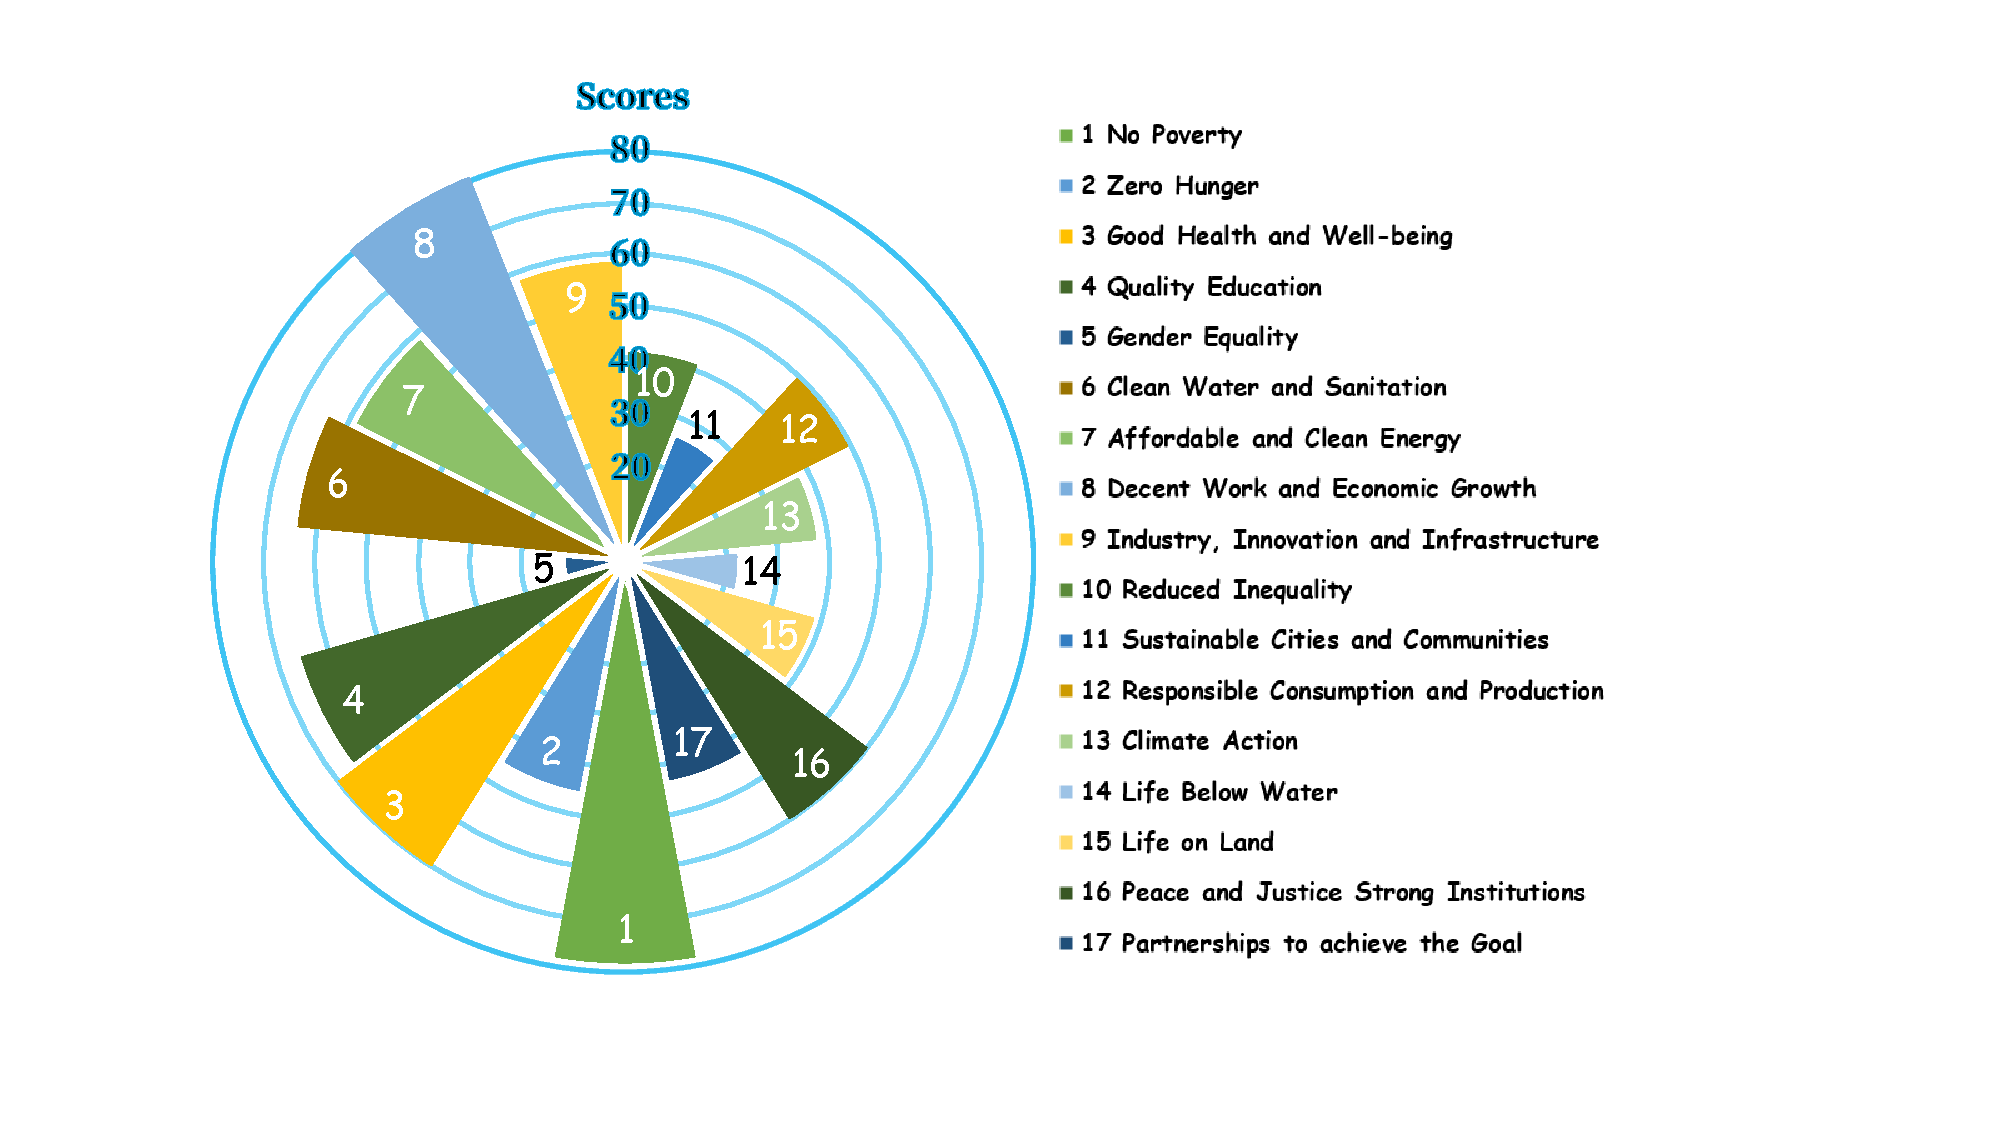
\includegraphics[width=.75\textwidth]{rank.pdf}
\caption{Prioritization of the 17 Sustainable Development Goals}\label{fig:4.2}
\end{figure}


As demonstrated in Figure \ref{fig:4.2}, the Decent Work and Economic Growth(Goal 8) has the greatest positive impact on the overall network, followed by Decent Work and Economic Growth(Goal 8) and Good Health and Well-being(Goal 3), which are all indicators of the economy and people's livelihood.
We attribute China's better performance on economic goals 11, 8, and 1 to the following reasons:
\begin{itemize}
\setlength{\itemsep}{0pt}
\setlength{\parsep}{0pt}
\setlength{\parskip}{0pt}
    \item 
China has implemented several policies such as urban regeneration projects, reforms to urban planning and development regulations, and investments in public transportation infrastructure.
\item The Chinese government has also implemented reforms to the labor market and relaxed restrictions on foreign investment in order to further support economic growth.
\item The Chinese government has launched poverty alleviation initiatives, such as the “Targeted Poverty Alleviation Program”, to reduce the number of people living in extreme poverty.
\end{itemize}
Additionally, it has also been  observed from Figure \ref{fig:4.2} that China's performance in humanistic indicators, such as Gender Equality, and environmental indicators, such as Life Blow Water, is not satisfactory. 
We attribute China's poor performance on these indicators to the following reasons:
\begin{itemize}
   \setlength{\itemsep}{0pt}
\setlength{\parsep}{0pt}
\setlength{\parskip}{0pt}
\item[*] Poor enforcement of environmental regulations, low public awareness of environmental issues, and scarcity of resources and technology exacerbate environmental pollution.
\item[*] China's rapid economic growth and industrialization have also contributed to the country's poor performance in this goal. 
\end{itemize}

\subsubsection{Analysis of the Implementation of Prioritization}
%%%%%%%%%2

\vspace{0.7mm}\begin{itshape}
\textbf{$\blacktriangleright$
Community Detection
}\end{itshape}


The algorithm of community detection divides certain interrelated nodes into a community, and the nodes in each community are categorized into one of the Sustainable Development Goals (SDGs): economic, social, and ecological. The size of each node is a calculated score representing its ability to promote the entire SDG, while the color of the node denotes the category it has been divided into by the community detection.
Figure \ref{fig:4.3} presents the Sustainable Development Goals Network based on Community Detection.
%%%%%%%%%%%%%%%%%%%%%%%%%%%%%%%%%%%%%%%%%%%%%%%%%%%%%%%%%%%%%%%%%%%%%%%%%%%%%%%%%%%%%%%%%%%%%%%%%%%%%%%%%%%%%%%%%%%%%%%%%%%%%%%%%%%%%%%%%%%%%%%%%%%%%%%%%%%%%%%%%%%%%%%%%%%%%%%%%%%%%%%%放一张图片就行

\begin{figure}[htbp]
\centering
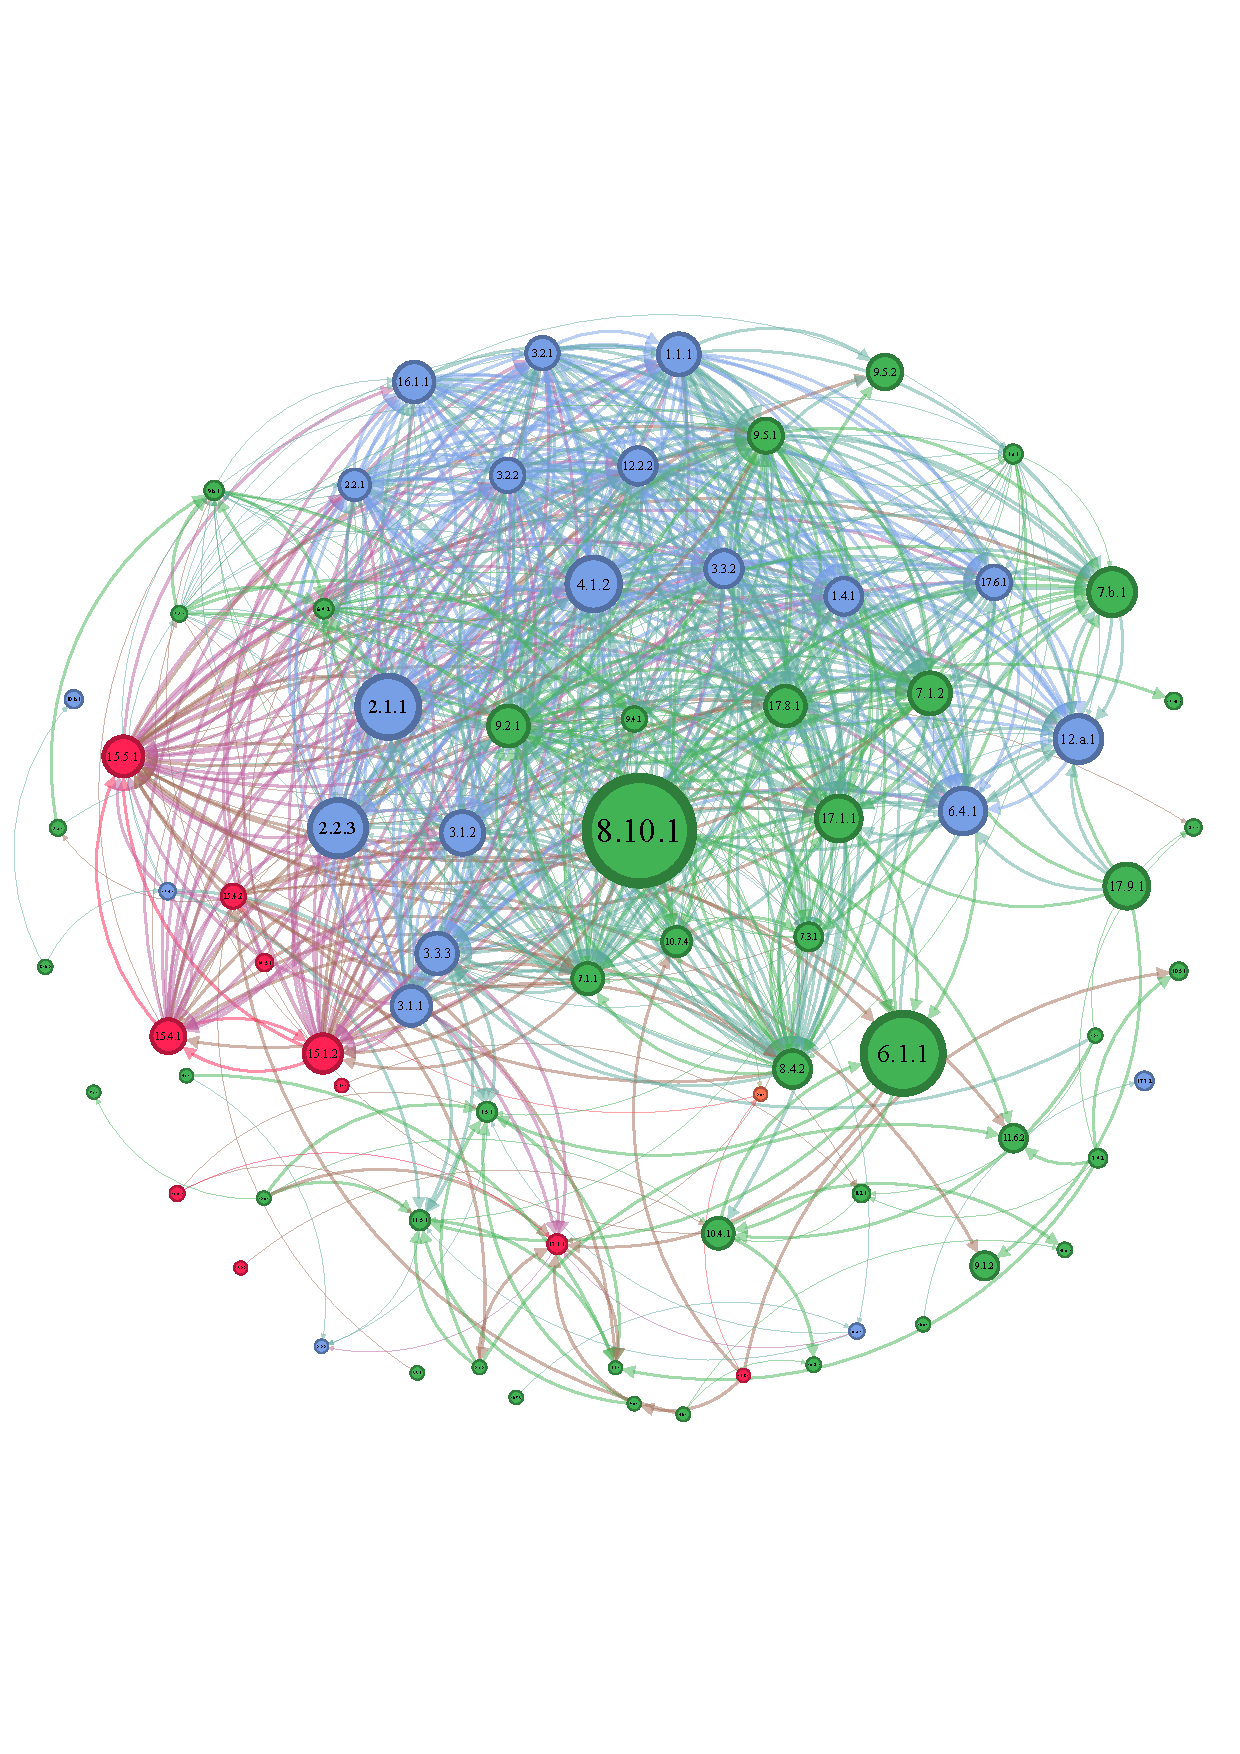
\includegraphics[width=.5\textwidth]{community.pdf}
\caption{Sustainable Development Goals Network based on Community Detection}\label{fig:4.3}
\end{figure}

In the network, the indicators of the green category roughly belong to the goals in the Sustainable Development Goals (SDGs) 7, 8, 9, 10 and 17. These metrics are classified as economic; the size of a node thus represents the economic influence of that metric on the network. Node 8.10.1 is the largest node in the economic category, and its corresponding indicator is the number of commercial bank branches available per 100,000 adults. This implies that to promote economic development in the region, we need to increase the number of commercial bank branches available per 100,000 adults, thus enabling more people to storage their property conveniently. 


The indicators represented by the blue nodes belong to the Sustainable Development Goals (SDGs) 1, 2, 3, 4, and 16, and are indicators of sustainable development of society. The node corresponding to the 2.1.1 indicator is particularly large, indicating the need to increase the incidence of undernourishment in order to reduce hunger, which is the prerequisite for people to enjoy a happy life and good employment. The realization of these nodes is thus conducive to promoting the sustainable development of the entire network society.

\vspace{0.7mm}\begin{itshape}
\textbf{$\blacktriangleright$
Validation of Prioritization 
}\end{itshape}

According to our ranking,  no Hunger(Goal 8) and  Employment and Economic Growth(Goal 1) should be achieved first, which is also in line with China's national strategy. All poverty-stricken counties will be lifted out of poverty, and a moderately prosperous society will be achieved in 2020.  However, due to the impact of the COVID-19,  employment in China is projected to be depressed in 2022, and the economic growth rate will decline. This necessitates urgent measures to create jobs and grow the economy, thus proving that our priorities are consistent with the national development strategy, demonstrating the effectiveness of the established model.


\vspace{0.7mm}\begin{itshape}
\textbf{$\blacktriangleright$
Prediction of Achievements}\end{itshape}

The Venn Diagram is a useful tool for Social Network Analysis (SNA) as it allows for a visual representation of the relationships between entities. It enables the user to gain a better understanding of the structure of the network by providing a clear overview of the connections between nodes\upcite{2}. 
Drawing on the three dimensions of society, environment, and economy proposed by the Venn Diagram, and the priority levels provided in Figure \ref{fig:4.3}, we describe the achievements and changes that SDGs have brought to China from the perspectives of society, environment, and economy.


\textbf{$\bullet$ Economy Dimension:} If the sustainable development goals are achieved in the order given, it is likely that the Chinese economy, society, and environment will all benefit. Economically, Decent Work and Economic Growth will create more job opportunities and increased income, Industry, Innovation and Infrastructure will drive economic growth, and Affordable and Clean Energy will reduce energy costs and pollution. 

\textbf{$\bullet$ Society Dimension:} Socially, Good Health and Well-being will result in improved health outcomes, Quality Education will provide increased access to quality education, Reduced Inequality will reduce inequality and poverty, and Gender Equality will ensure equal rights and opportunities. 

\textbf{$\bullet$ Environment Dimension:} Environmentally, Sustainable Cities and Communities will lead to better urban living conditions, Clean Water and Sanitation will lead to improved water quality, Life on Land will protect wildlife and natural habitats, Climate Action will reduce carbon emissions, and Life Blow Water will improve water quality.

\section{\textsc{Task 3:} Derived Subgraph of the Sustainable Development Goals Network}
\subsection{Model Overview}

In \textsc{Task 3}, we aim to analyze the impact of the partial achievement of the SDGs on the overall network. The realization of the sustainable development goals can be understood as the corresponding network nodes and their associated edges being removed, resulting in a new network graph which can be regarded as the network graph of the 17 sustainable development goals. Sub-graphs can be exported from this new network graph. The centrality index and influence index of the sub-network can then be calculated to obtain a new priority ranking of network nodes.
\subsection{Derived Sub-graph of the Sustainable Development Goals Network}
When the goal of No Poverty has been achieved, the corresponding indicators are removed and the related network nodes and edges associated with them are also removed. This results in the newly established network being equivalent to the derived sub-graph of the original network, as shown in the following figure:


At the same time, we solved the established Dual-Strategy Sustainable Development Goals Network again, obtaining the scores corresponding to the remaining 16 goals and comparing them with the priority scores before implementing no poverty. This revealed the following changes:

$\bullet$
The scores of Zero Hunger (Goal 2) and Decent Work and Economic Growth (Goal 8) dropped the most, both decreasing by approximately 30 points. This indicates that the priority of both Goal 2 and Goal 8 has been significantly reduced, which is in line with our previous analysis.
% When the alignment between two targets is strong, the buff of one target will push the buff of the other target and thus reduce the priority of the affected target. This implies that it has grown significantly, and there is much less need and urgency to continue developing. 
From the perspective of Goal 1 and Goal 2, after No Poverty has been achieved, individuals can obtain food and money that meets their basic needs, which will help towards achieving the goal of Zero Hunger. At this time, the marginal effect of developing Goa l 2 begins to diminish, thus reducing its priority score. Similarly, the realization of Goal 1 also means that the employment rate has steadily increased, and the resulting human resource dividend has promoted the development of the entire country's economy and achieved a higher level of economic productivity. As a result, the marginal effect of Goal 8 will also decrease, thus decreasing its priority score.

$\bullet$ In addition to Goal 2 and Goal 8, the scores of Goal 3, 4, 7, 9, 11,  12 and 16 have also been reduced to varying degrees. And these indicators are consistent with Goal 1, that is, the realization of Goal 1 can promote the realization of these goals to a certain extent. We choose Goal 4 for typical analysis. When no poverty is achieved, the education level of the population will continue to increase, and the higher education acceptance rate will also increase. In this way, the priority of Goal 4 will also be reduced, but the impact of no poverty on quality education is indirect, so the degree of score drop is not as good as Goal 2 and Goal 8.

$\bullet$ The priority scores of Goal 6 and Goal 13 have both been improved by more than 25 points, which happens to be in the opposite direction to the change direction of Goal 2 and Goal 8. For Goal 2, after the poverty problem is solved, the people's quality of life will be improved, and the improvement of the level of economic development will bring some environmental pollution in the initial stage. Besides, the improvement of living standards will also be accompanied by the derivation of unreasonable consumption habits, including the waste of water resources, so the realization of no poverty is not conducive to the advancement of Clean Water and Sanitation. In the same way, for Goal 13, the improvement of economic level brings about the promotion of social industrialization process, and at the same time, it will cause the emission of carbon dioxide and harmful gases, which are all factors that are not conducive to the realization of Climate Action. In order to achieve sustainable development, we should increase the priority of these two goals, so the priority score has been greatly improved.

$\bullet$
In addition to the above goals, there are still a lot of goal scores that basically remain unchanged or slightly increase, such as Goal 5, 10, 14, 15 and 17. These goals are basically not very related to the realization of Goal 1, but due to Goal 1 has a great positive influence, the number of promoting goals is far greater than that of counteracting goals, that is, among the goals related to Goal 1, the priority scores are lowered in the majority. Therefore, the priority scores of the remaining goals whose relationship with Goal 1 is not obvious will remain unchanged or even slightly increased.
\subsection{Dynamic Adjustment of Network Nodes}
After the realization of No Poverty Goal, the priorities of goals 2, 3, 4, 7, 8, 9, 11, 12, and 16 are reduced, and corresponding progress is made under its positive promotion, especially Goal 2 and 8 are developing rapidly. The priorities of Goal 6 and 13 are raised, which means the realization of no poverty inhibits their development to a certain extent.

$\bullet$ \textbf{Overall Prosperity:} The realization of No Poverty has had a significant impact in promoting more than half of the goals. Moreover, when considering the secondary effects of the goals positively promoted by Goal 1, it is evident that the positive influence of Goal 1 is closely linked to the overall situation. For this reason, we propose the introduction of another goal that is consistent with the direction and connotation of No Poverty: Overall Prosperity. Overall Prosperity and No Poverty are interrelated and internally consistent, and are the result of the continuous advancement and gradual progress of Goal 1. The goals corresponding to Overall Prosperity include living expenses of not less than US\$3 per person per day, implementation of national social security systems and measures suitable for the country’s national conditions and covering all citizens, and so on.

$\bullet$ \textbf{Harmonious Coexistence Between People and Nature:} While analyzing the positive impact of the realization of no poverty, we should pay more attention to the Goal 6 and 13 that are suppressed by it. Based on this, we propose to introduce the goal of "Harmonious Coexistence Between People and Nature", which emphasizes the relationship between man, environment and ecology. The targets included include: all very wild and individuals should improve the utilization efficiency of natural resources such as water and natural gas, and strictly protect them. Ecosystems such as forests and rivers, strict management of the discharge of various pollutants, adherence to low-carbon life, etc. The introduction of harmonious coexistence between people and nature can largely compensate for the negative impact of Goal 1 on Goal 6 and 13, which is conducive to the full realization of all goals.




\section{\textsc{Task 4:} Dynamic Sustainable Goals Network \& Its Extensions}
\subsection{Model Overview}
Task 4 necessitates the consideration of the impacts of changes in the external environment on network structure. To carry out analysis based on the actual situation in the selected regions, we measure the degree of alignment of SDGs with society, establish and quantify a consistency indicator. We select the global pandemic  as an influencing factor,  and adjust the weight of the network by altering the degree of alignment of SDGs with society.
\subsection{Establishment of Dynamic Sustainable Goals Network}
% \subsubsection{Assessing Alignment of SDGs with Society}


\vspace{0.7mm}\begin{itshape}
\textbf{$\blacktriangleright$ Assessing Alignment of SDGs with Society}\end{itshape}


% Owing to the region and the resources available,
The seventeen goals of the SDGs have different levels of implementation in China. 
This paper evaluates the actual realization and implementation of each Sustainable Development Goals, dividing them into four categories. Then the assessment is then mapped to a numerical value via a simple additive scoring method\upcite{7}.


Through evaluating China's performance on the seventeen interdependent goals, we can assess the effectiveness of the SDGs implementation and determine the priority of the nodes.  
Green, yellow, orange, and red signify the difficulty in achieving the corresponding Sustainable Development Goals (SDGs) in China, with green indicating the lowest difficulty and red indicating the highest, which is shown in Table \ref{tab:6.1}.
\begin{center}
\begin{table}[!htbp]\vspace{-1.5em}\centering\caption{China's Performance on the SDGs}\label{tab:6.1}\begin{threeparttable}
\begin{tabular}{ccccccccc}
\toprule[1pt]
\textbf{SDG1} & \textbf{SDG2} & \textbf{SDG3} & \textbf{SDG4} & \textbf{SDG5} & \textbf{SDG6} & \textbf{SDG7} & \textbf{SDG8} & \textbf{SDG9} \\ 
% \midrule
% \specialrule{0em}{1.5pt}{1.5pt}
\hline
\cellcolor{Yellow} Y & \cellcolor{BurntOrange} O &\cellcolor{BurntOrange} O &\cellcolor{LimeGreen} G & \cellcolor{BurntOrange} O & \cellcolor{BurntOrange} O &\cellcolor{BurntOrange} O &\cellcolor{LimeGreen}  G & \cellcolor{BurntOrange}O \\ \hline
\textbf{SDG10} & \textbf{SDG11} & \textbf{SDG12} & \textbf{SDG13} & \textbf{SDG14} & \textbf{SDG15} & \textbf{SDG16} & \textbf{SDG17} & \\ \hline
% \specialrule{0em}{1.5pt}{1.5pt}
% \midrule
\cellcolor{Red} R & \cellcolor{BurntOrange} O & \cellcolor{BurntOrange} O &
\cellcolor{Red} R &
\cellcolor{Red} R & \cellcolor{BurntOrange} O &
\cellcolor{Red} R & \cellcolor{BurntOrange} O & \\ \hline
\end{tabular}

\end{threeparttable}\begin{tablenotes}
\footnotesize
\item[1] G(reen): SDG Achievement; Y(ellow): challenges remain; O(range) Significant challenges remain; R(ed) major challenges\upcite{7}.
\end{tablenotes}\vspace{-1.5em}
\end{table}\end{center}

To quantify China’s performance on the 17 goals for prioritizing network nodes, we map G, R, O, and R to $0$-$1$ to develop a Consistency Index $CI_i$. 
Assuming China's performance efficiency in the $i$-th goal is $Goal_i$, and its discret
 values are G, R, Y, O.
Let the selected indicator be $a_i$, and the set of all indicators included in Goal $i$ be $Goal_i$. Then the indicator $a_i$'s  Consistency Index   $CI_i$ is given by the following:
\begin{equation*}CI_i=
\begin{cases}0.25,\quad &i\in Goal_j\& Goal_j=G,\\0.5,\quad &i\in Goal_j\&Goal_j=Y,\\0.75,\quad &i \in Goal_j\&Goal_j=O,\\1,\quad &i \in Goal_j\&Goal_j=R.
\end{cases}
\end{equation*}
% \subsubsection{Impact of the Global Pandemics}

\vspace{0.7mm}\begin{itshape}
\textbf{$\blacktriangleright$ Impact of the Global Pandemics}\end{itshape}

The COVID-19 pandemic has exerted immense pressure on the world economy and business operations, resulting in substantial financial repercussions, as well as exacerbating poverty and hunger worldwide, hindering progress towards sustainability. This jeopardizes our capacity to accomplish many of the 17 Sustainable Development Goals as outlined in the 2030 Agenda, while diminishing the significance of the SDGs for the world’s governments\upcite{10}. 

% This information would allow a better comprehension of the actual state of the SDGS and
% more efficient programming in future interventions


The impact of the COVID-19 pandemic on the SDG goals is mainly focused on the following aspects:

\begin{itemize}
   \setlength{\itemsep}{0pt}
\setlength{\parsep}{0pt}
\setlength{\parskip}{0pt}
    \item \begin{itshape}
        \textbf{Good Health and Well-being:}
    \end{itshape}  The COVID-19 pandemic has caused significant disruption to global health systems, as the virus has spread rapidly and hindered access to essential health services, including in areas such as mental health, sexual and reproductive health, and drug-resistant infections.  \item \begin{itshape}
        \textbf{Sustainable Cities and Communities:}
    \end{itshape} The COVID-19 pandemic has caused significant disruption to global infrastructure and urban development projects, resulting in a decrease in access to housing and public services, as well as a decline in economic activity. 
\end{itemize}

In order to demonstrate the importance of the influence of these two goals, we double the value of the alignment of Goal 3 and Goal 11. 


\subsection{Analysis of the Results}

Figure \ref{fig:6.1} illustrates the dynamic ranking changes of China’s SDG network after the COVID-19 epidemic; the numerical numbers of the nodes correspond to the goal numbers; the color of the nodes indicates the category to which the goal belongs (red represents ecology, blue represents society, and green represents economy).

\begin{figure}[htbp]
\centering
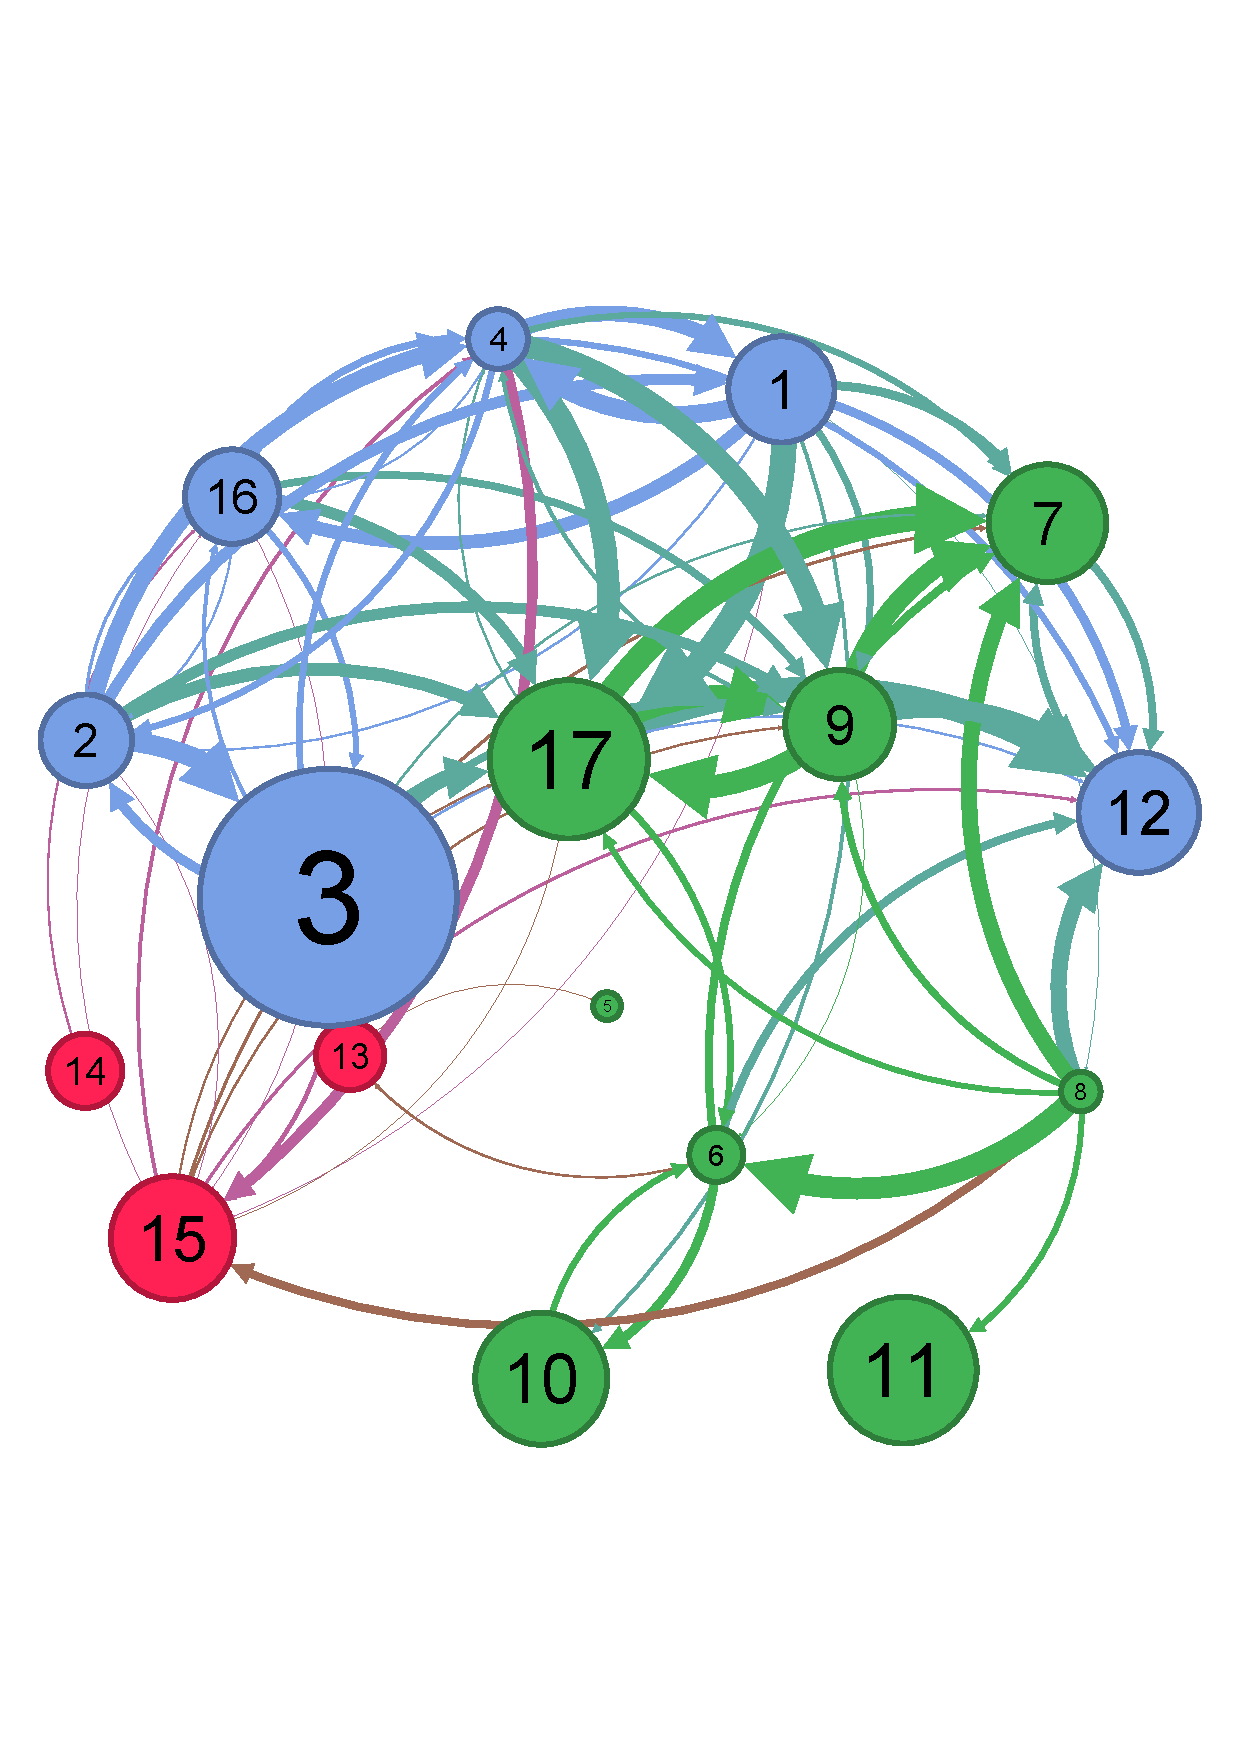
\includegraphics[width=.5\textwidth]{pandemic.pdf}
\caption{Sustainable Development Goals Network with Global Pandemic}\label{fig:6.1}
\end{figure}


As seen in Figure \ref{tab:6.1}, the size of node 3 and node 11 is relatively large, which is in accordance with our adjustment of the Consistency Index of Goal 3 and Goal 11 in the model. The number of edges between each goal node is reduced and the weight is also significantly decreased, indicating that the COVID-19 epidemic has hindered the UN's sustainable development goals agenda.

By comparing the priority scores of each goal before and after the introduction of the COVID-19 epidemic, we justify the introduction of the consistency index. It can be clearly seen from the radar map that, after the impact of the novel coronavirus epidemic, the priority scores of Goal 3 and Goal 11 are surprisingly improved, while most of the other goals' priority scores are slightly decreased or remain unchanged. Therefore, the introduction of consistency index is reasonable. 

Differences in national conditions of different countries will lead to different grades of the 17 goals, that is, differences in priorities are also caused by Consistency Index. All in all, the model with consistency index has wider applicability and stronger robustness.

\begin{figure}[htbp]
\centering
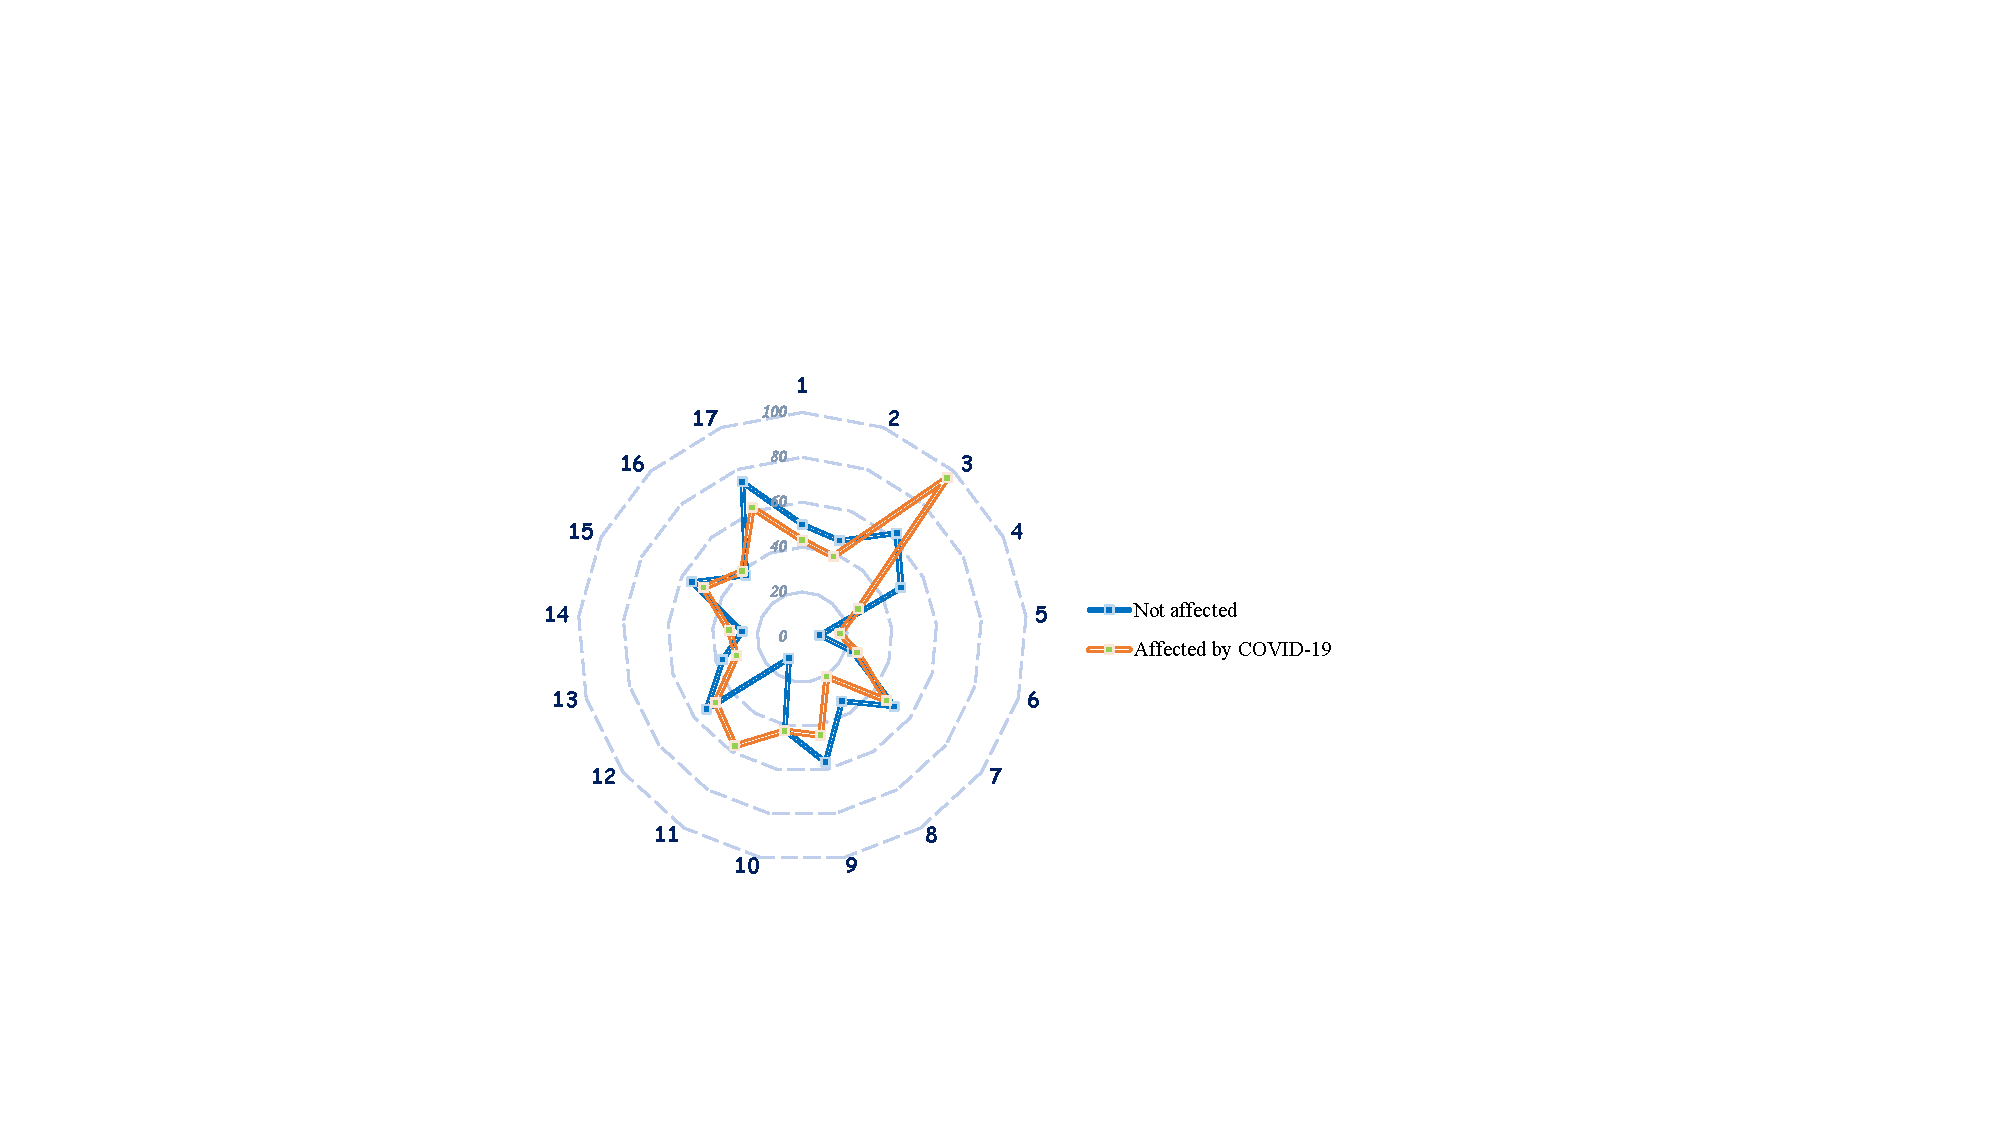
\includegraphics[width=.75\textwidth]{rado.pdf}
\caption{Radar Map of Sustainable Development Goals Prioritization Before and After COVID-19}\label{fig:6.1}
\end{figure}

\subsection{ Expansion of the Sustainable Development Goals Network}

The network we have constructed is an effective means of addressing the way industries prioritize goals, and it encourages departments to move beyond their silos and think systematically about their impact on and interactions with other departments. 

 Our network is also applicable for other companies and organizations to determine the priority of their goals. Once all the goals of the company are clarified, we can use the indicator data corresponding to each goal to analyze the interaction between goals or indicators, or through company management. The layer quantifies the mutual promotion relationship between various goals in numbers.
When the indicator data is incomplete, the interdependent relationship between various goals can also be quantified by the company's management. 


In \textsc{Task 2}, we established the Network Centrality Strategy and the Influence Strategy. In \textsc{Task 3}, the Consistency Index was introduced to measure the implementation effect of the SDG goals. Having obtained the interaction relationship between each node, we then combine the aforementioned three strategies into  in order to jointly determine the priority of the goal.
% \subsection{Criteria One: Assessing Network Centrality of Goals}

\vspace{0.7mm}\begin{itshape}
\textbf{$\blacktriangleright$
Criteria One: Assessing Network Centrality of Goals
}\end{itshape}

The impact of goal priority can be determined by discussing network centrality. %In the second question, we describe and weight network centrality from three perspectives: degree centrality, proximity centrality, and betweenness centrality. 
More other measures of centrality can be introduced, such as eigenvector centrality, Katz centrality, alpha centrality\upcite{6}. 
The entropy weight method can also be used to determine the weight of these network centrality indicators, and finally a comprehensive network centrality score is obtained.


The calculated score based on this strategy, can be used to evaluate the influence of a particular indicator within the whole network.
% \subsection{Criteria Two: Assessing  the Impact of Individual Goals}

\vspace{0.7mm}\begin{itshape}
\textbf{$\blacktriangleright$
Criteria Two: Assessing  the Impact of Individual Goals
}\end{itshape}

The influence of each goal can reflect its effectiveness in promoting the achievement of other goals when set as a priority, as well as its impact on the overall network structure when deleted. Furthermore, we accounted for the second-order network effects, i.e. how the affected goal further influence the goals around it, thus extending the influence of the original target and obtaining an effect on the entire network performance when a goal is prioritized.

% \subsection{Criteria Three: Assessing the Impact of Organizational Strategy on Goals Prioritization}
\vspace{0.7mm}\begin{itshape}
\textbf{$\blacktriangleright$ Criteria Three: Assessing the Impact of Organizational Strategy on Goals Prioritization}\end{itshape}

This strategy can not only link the short-term work focus and strategic goals of companies and organizations with the determination of goals priorities, but also play a role in the face of the impact of global epidemics, climate change and other international events on target priorities. It has a good buffering effect, and regulates the determination of the target priority as a whole.

It is worth highlighting that through a series of analyses, we can find that some indicators are closely and positively correlated, which forming a cluster. When  an indicator in the cluster is given higher priority and develops faster, it will have a positive driving effect on the development of the entire cluster. This rule corresponds to the development of companies and organizations, and represents the collaboration between different departments or units corresponding to different goals. Responsibility for the policy areas of the various objectives that make up the clusters falls to different ministries. Therefore, bridges of collaboration need to be built between departments, and active linkages between the goals they are responsible for are good entry points to promote this goal, emphasizing shared interests across departments.

Our network also takes into account the situations when one or more of the goals are achieved in the short-term and long-term startup priorities, updating the priorities accordingly in order to realize the dynamic update of the priorities throughout the period and show excellent stability and robustness after network testing.

Overall, our network performs well in elucidating the interplay between goals and viewing firm and organizational goals as an indivisible whole. Achieving the goals requires the concerted efforts of all departments of the company and the organization, and the impact of the alignment.

\section{Analysis on Model's Sensitivity}
Based on the threshold of the network edge, the network structure can be significantly altered, consequently impacting the prioritization of the 17 goals. Furthermore, this can influence the analysis of the network properties, such as network centrality and total influence.  All of these have a direct bearing on the accuracy of the SDG Network model and its ability to predict the implications of a given goal. Table \ref{tab:3.1} shows the changes in the number of nodes and edges brought about by the change of the threshold. 
Figure \ref{fig:8.1} shows the changes in the network structure under the four different thresholds.
\begin{figure}[htbp]
\centering
\begin{subfigure}[b]{.35\textwidth}
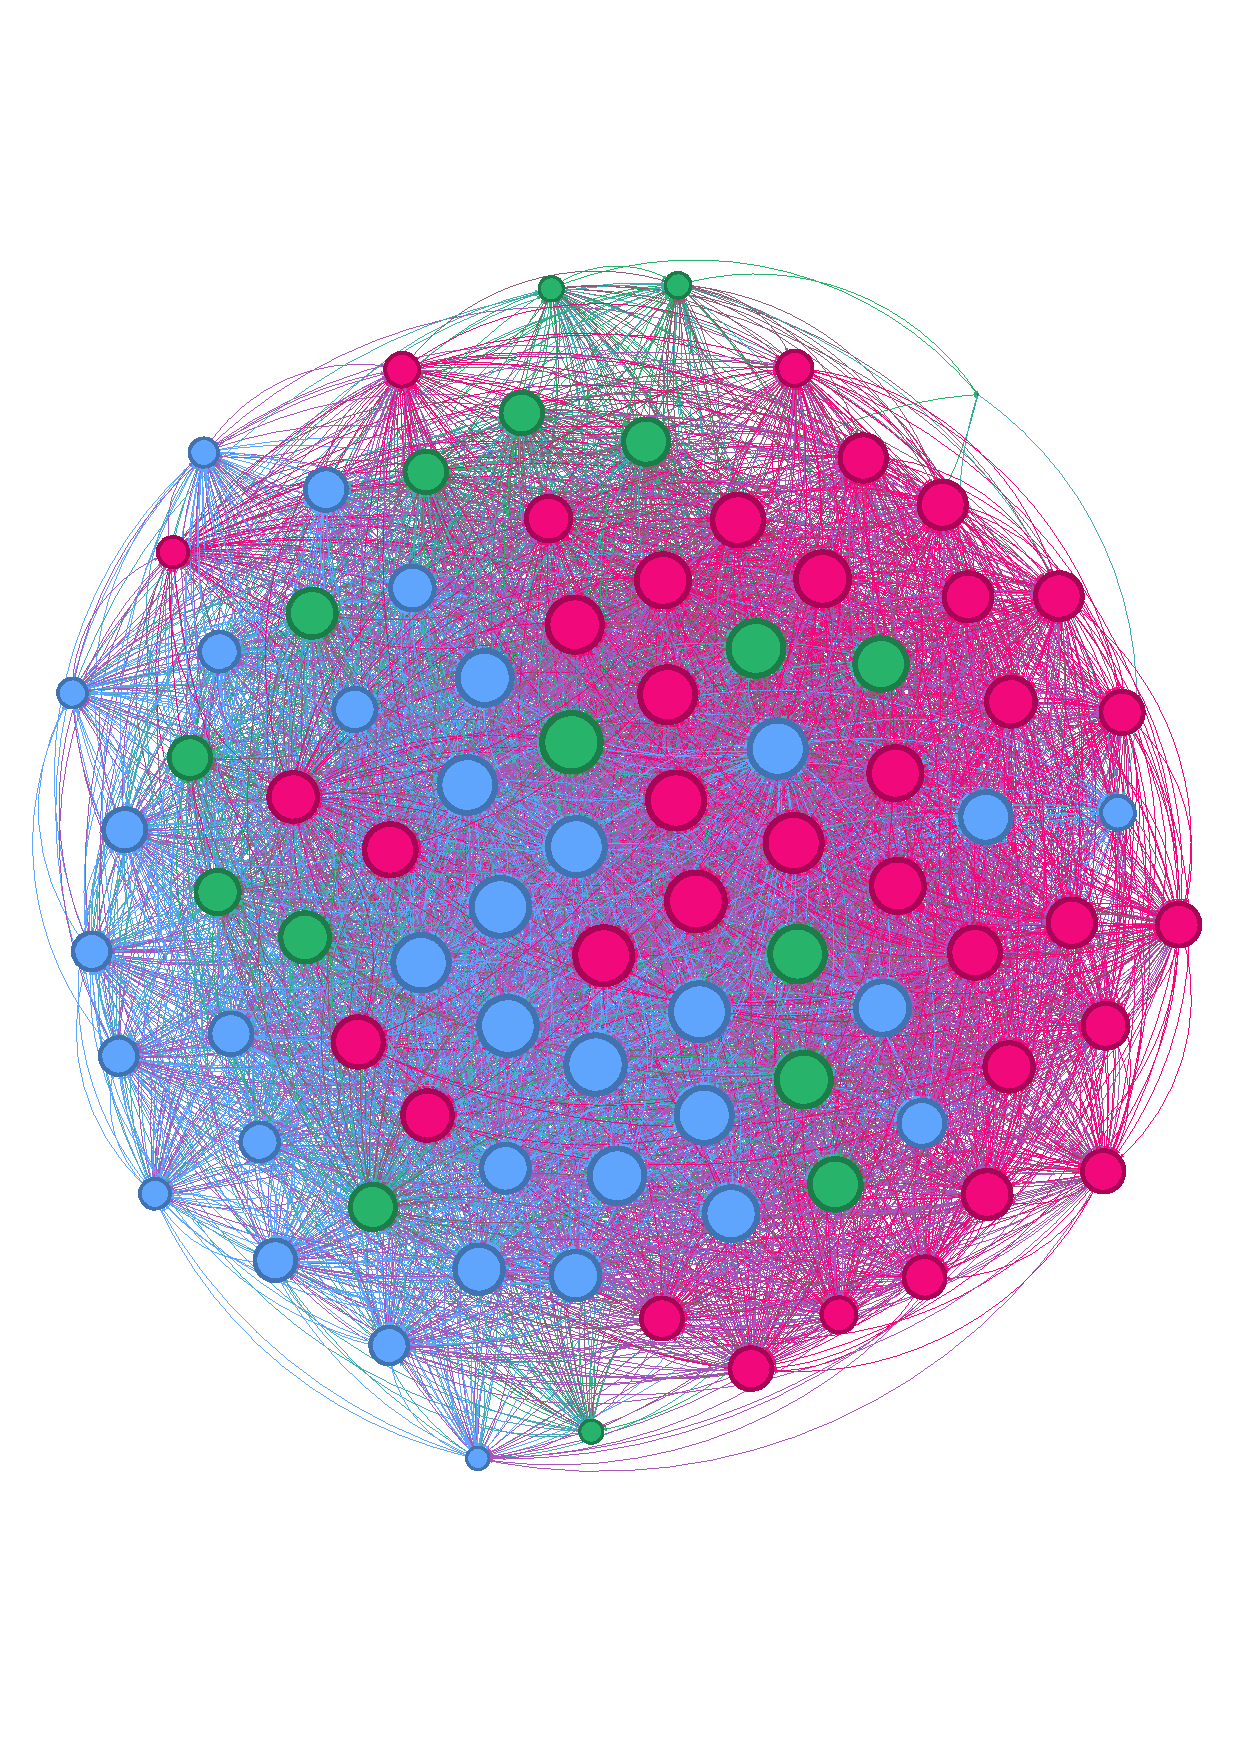
\includegraphics[width=\textwidth]{0.2.pdf}
\caption*{(a) $\sigma =0.2$}\label{subfig:left}
\end{subfigure}\qquad
\begin{subfigure}[b]{.35\textwidth}
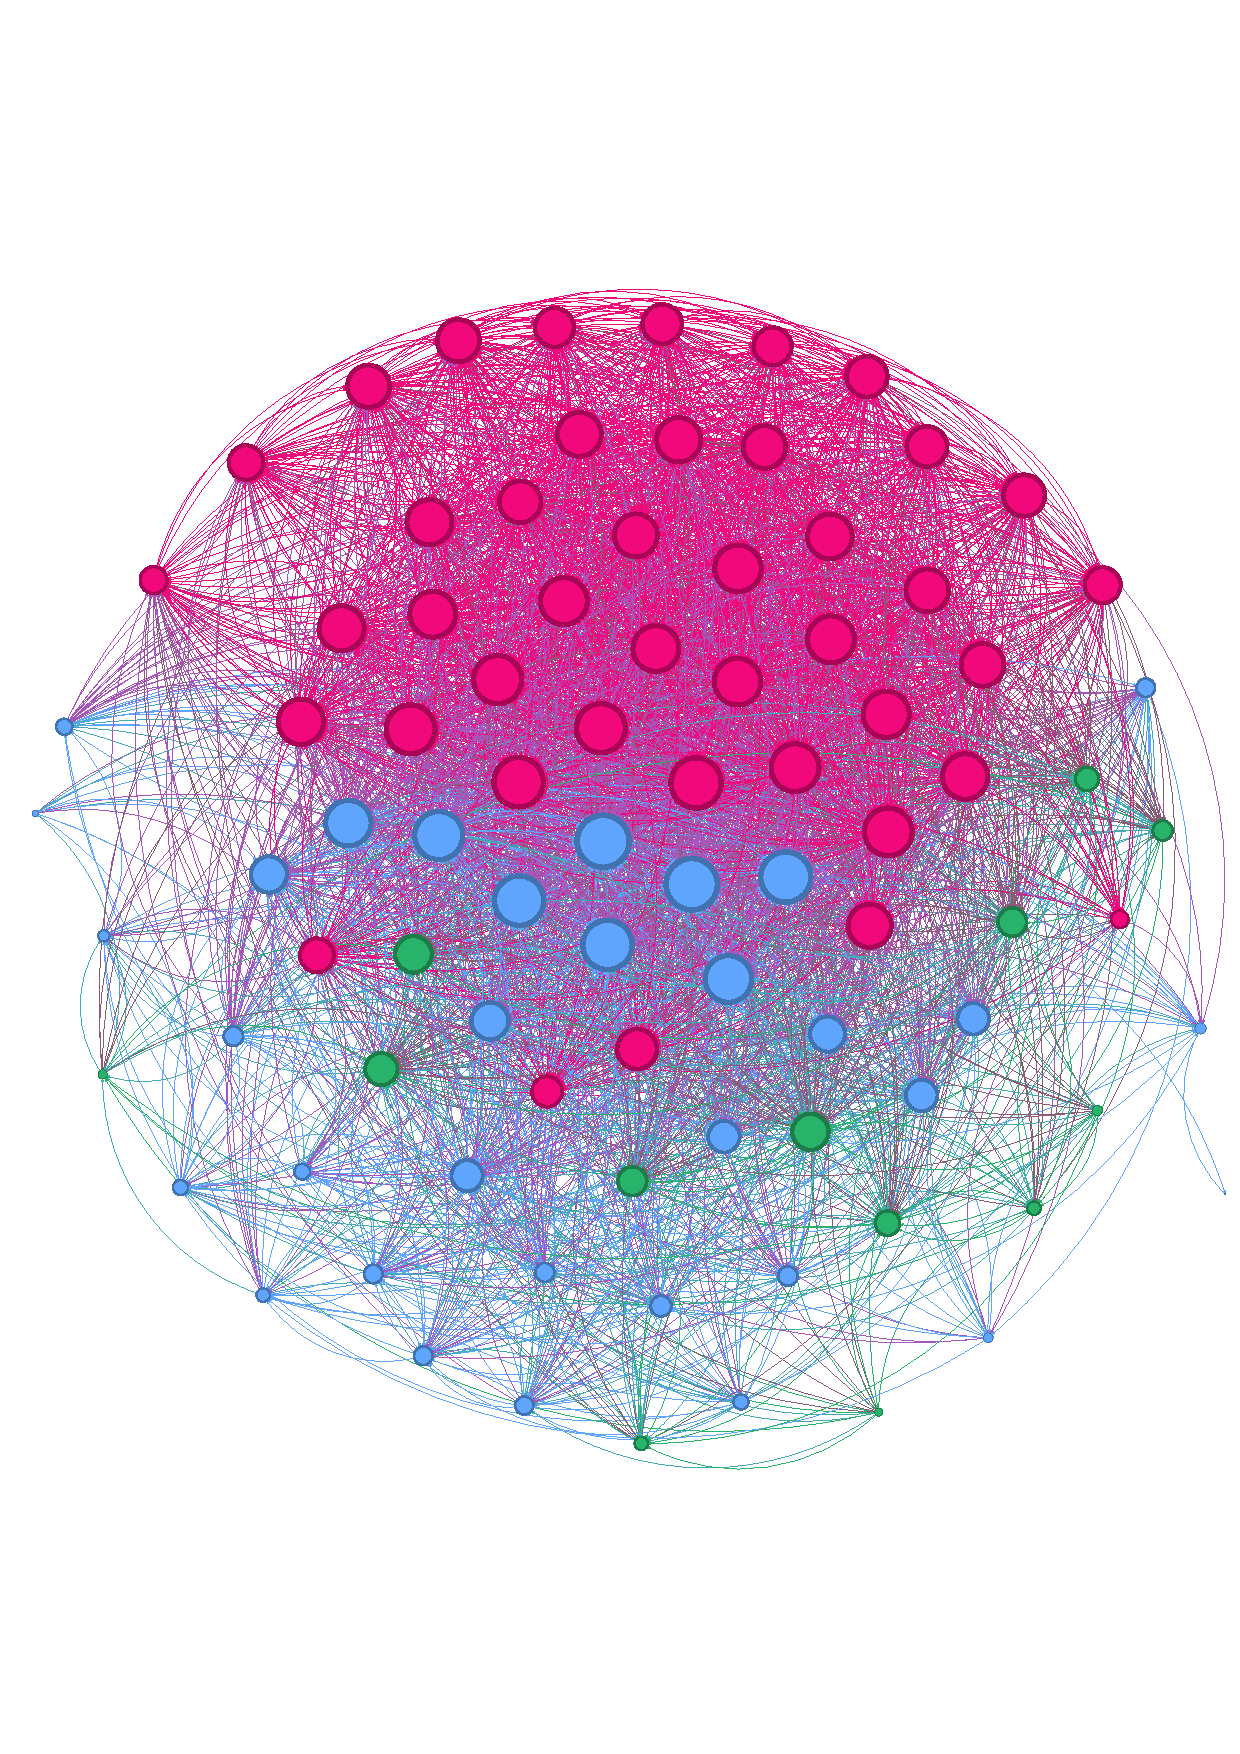
\includegraphics[width=\textwidth]{0.4.pdf}
\caption*{(b) $\sigma=0.4$}\label{subfig:right}
\end{subfigure}
\\
\begin{subfigure}[b]{.35\textwidth}
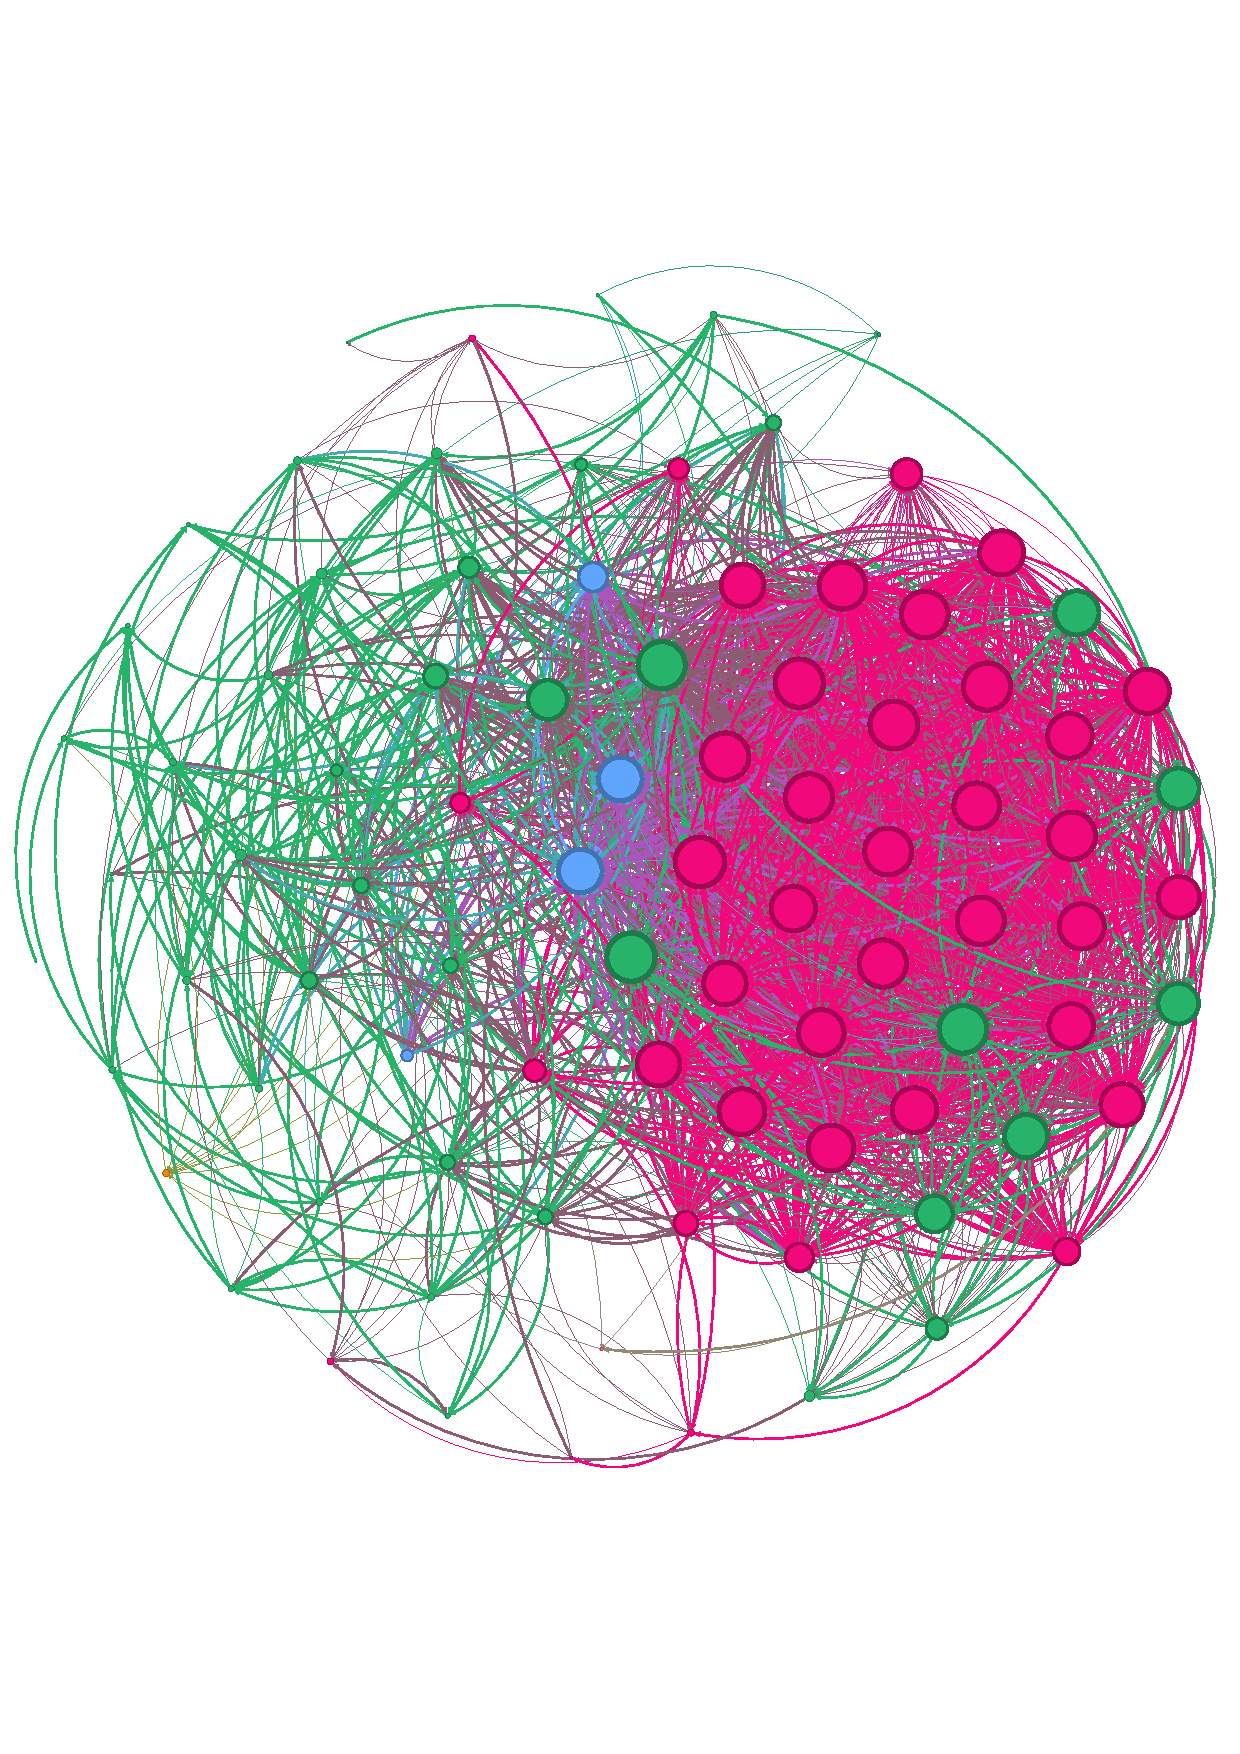
\includegraphics[width=\textwidth]{0.6.pdf}
\caption*{(c) $\sigma=0.6$}\label{subfig:left}
\end{subfigure}\qquad
\begin{subfigure}[b]{.35\textwidth}
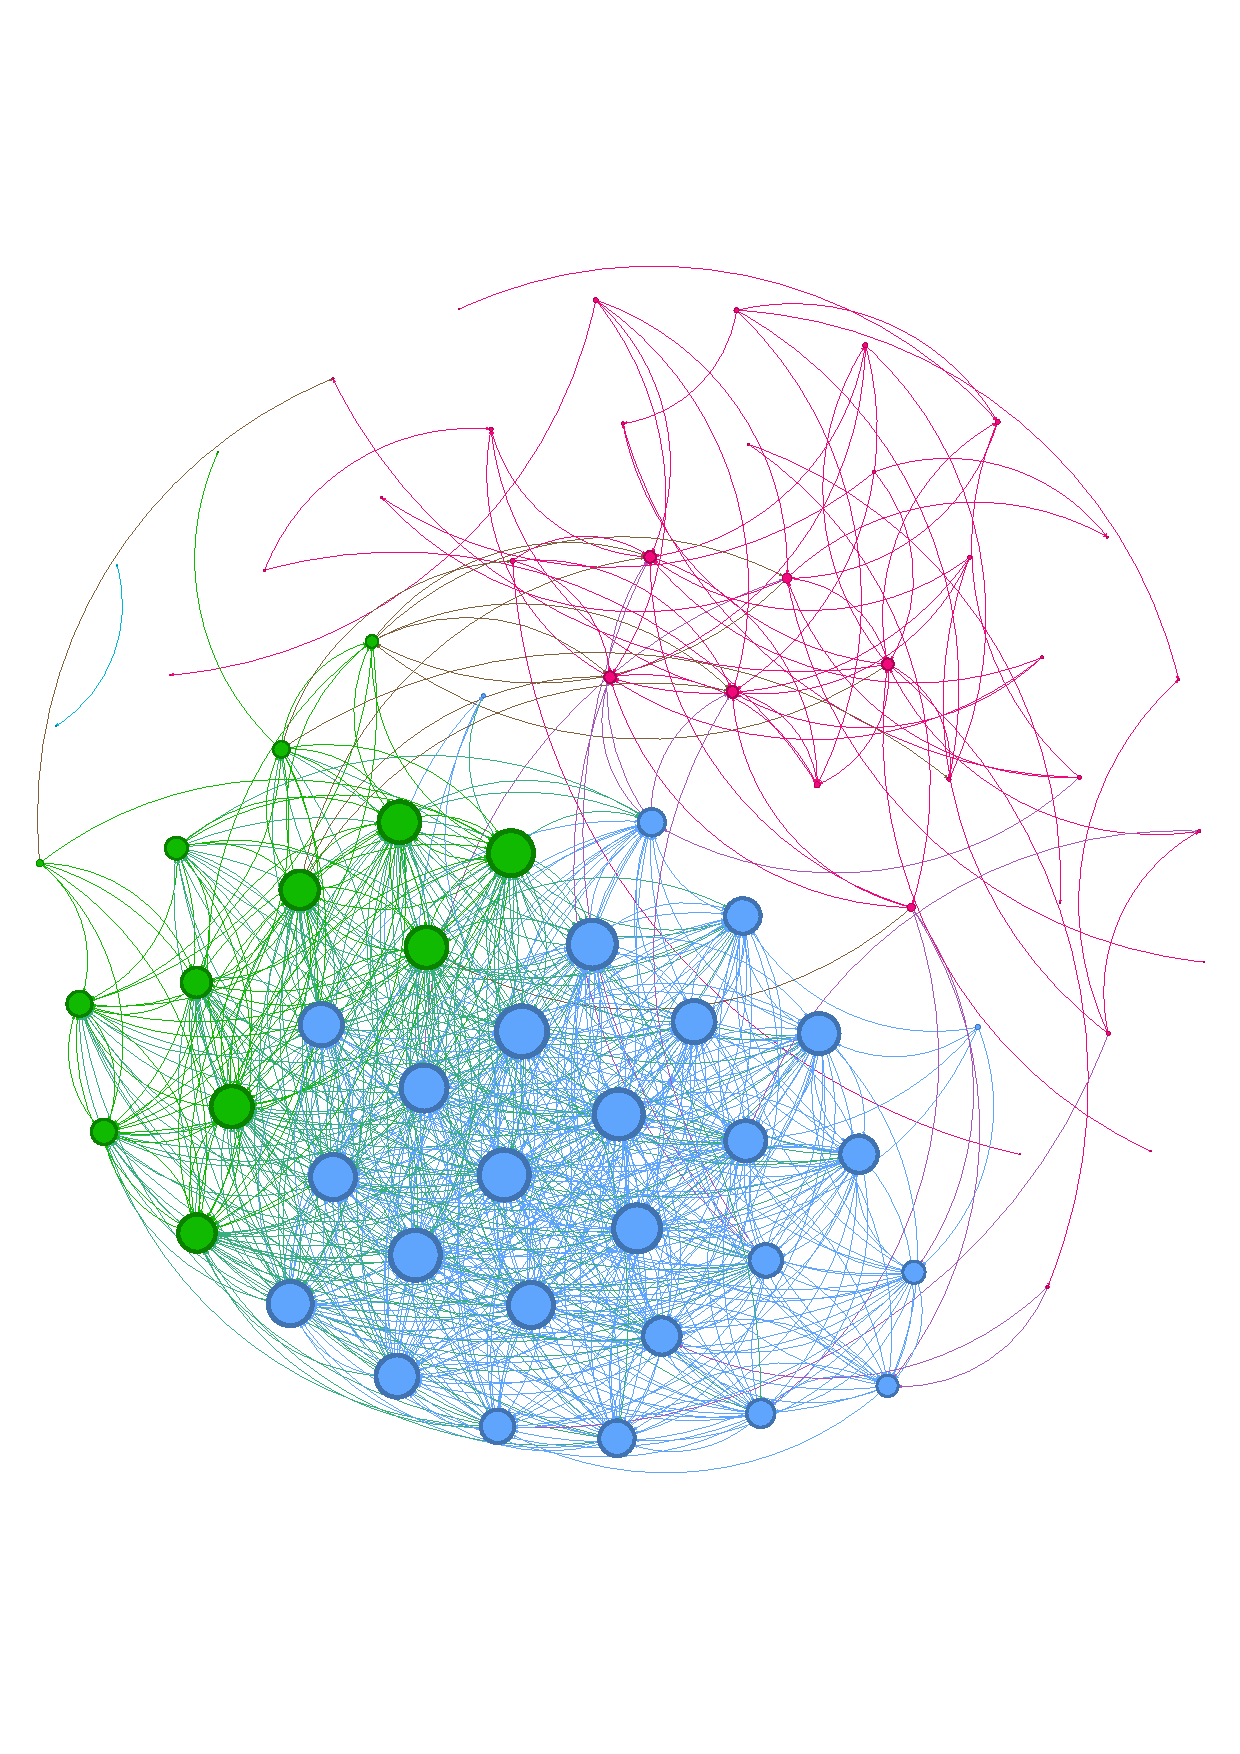
\includegraphics[width=\textwidth]{0.8.pdf}
\caption*{(d) $\sigma=0.8$}\label{subfig:left}
\end{subfigure}\caption{Sustainable Development Goals Network under Different Thresholds}\label{fig:8.1}
\end{figure}

Mathematically speaking, the higher the value of the threshold $\sigma$, the simpler the network structure and the more dense its edges. As seen in Figure \ref{fig:8.1}, as the value of $\sigma$ decreases, the network structure tends to become more complex. When  $\sigma$ is relatively small (for example, 0.2 and 0.4), the number of edges is particularly large, the connections between nodes are too frequent, and the relationship between networks is not obvious. When  $\sigma$ is 0.6, the clear structure of the network has begin to show slowly. When  $\sigma$ is 0.8, the weak connections in the network have been completely filtered, and the node relationships in the network are also very clear. Therefore, the threshold value should be 0.8.



\section{Strengths and Weaknesses}
\subsection{Strengths}
$\bullet$ We use the theory of SNA to construct a network of Sustainable Development Goals
to measure the interlinkages and priorities of indicators and  network with well-considered metrics.

$\bullet$ 
We take the second-order interaction into account, whereby the nodes that are affected can propagate the influence they receive in the network, thus making the impact of the original node on the network performance more comprehensive.

$\bullet$
We employ multiple strategies when assessing the priority of the goals, not only considering the mutual influence between the goals, but also taking into account the impact of the goals' consistency with the current situation and development strategy on the priority.

$\bullet$
We introduce the concept of clusters, and propose that the stakeholders of closely related goals should cooperate and promote one another, thereby facilitating the achievement of the goals through comprehensive thinking.


\subsection{Weaknesses}
$\bullet$ When processing indicator data in the same direction, we rely solely on human subjective judgments to determine whether the indicator is positive or negative. We should take into account that the nature of a country’s indicators is not static across different periods and scenarios.

$\bullet$ We could also go deeper into the analysis of certain issues, but due to space limitations,
we can only stop here.

$\bullet$ When building the network, we only select some indicators under each goal, and the description of the goal may not be complete and comprehensive.


\clearpage

\begin{subappendices}  % 附录环境

\section{Appendix: Tire Indicators of SDGs}
Since the space is limited, we have listed the metrics under the Tier of Goal 1 and Goal 17.
\begin{figure}[htbp]
\centering
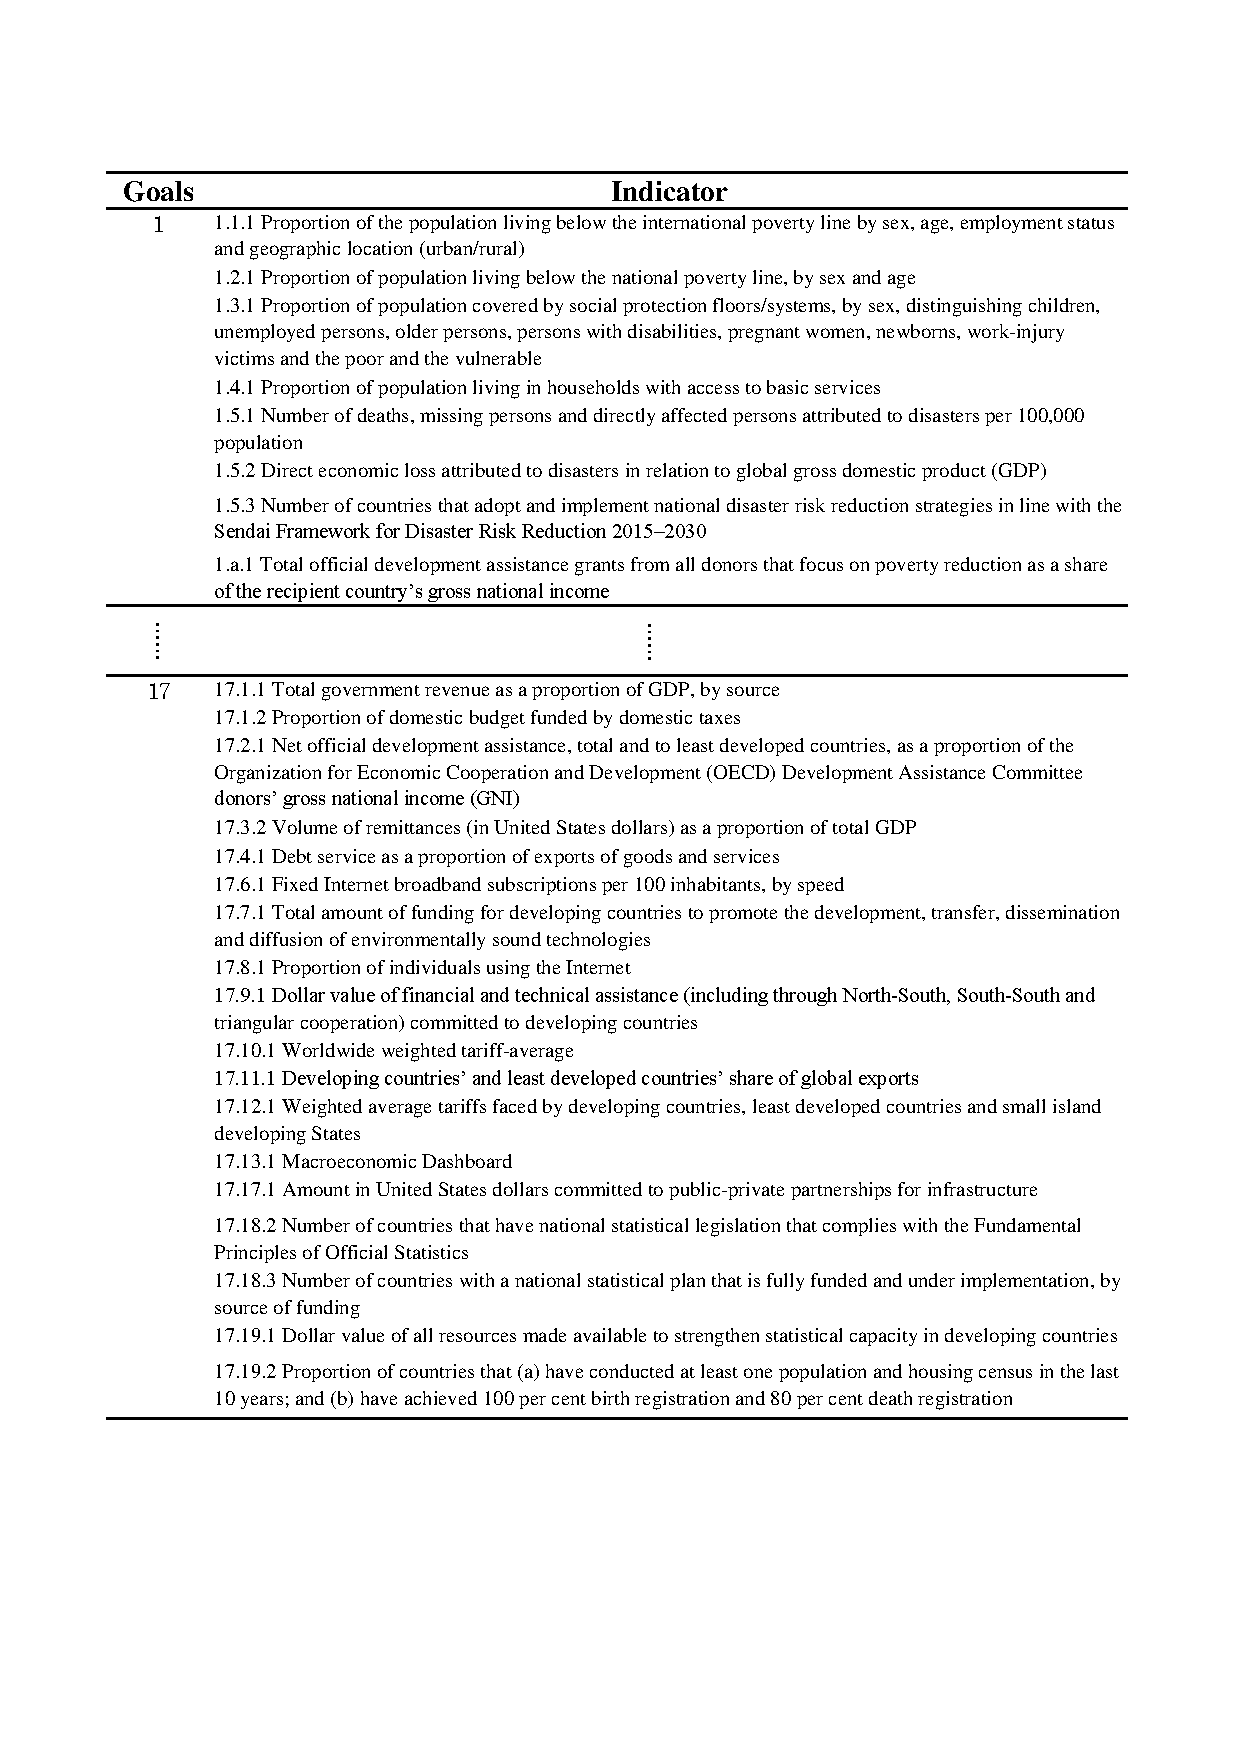
\includegraphics[width=.90\textwidth]{preparation.pdf}
\caption{Tier 1 Indicators of SDGs}
\end{figure}



\end{subappendices}







% \clearpage
% \subsubsection{Commetary on Model 2}
% The instance of long and wide tables are shown in Table \ref{tb:longtable}.

% % 长表格示例,更多用法请参考 longtable 宏包文档
% % 以下环境及对应参数可实现表格内的自动换行与表格的自动断页
% % 您也可以选择自行载入 tabularx 宏包,并通过 X 参数指定对应列自动换行
% \begin{longtable}{ p{4em} p{14em} p{14em} }
% \caption{Basic Information about Three Main Continents (scratched from Wikipedia)}
% \label{tb:longtable}\\
% \toprule
% Continent & Description & Information \\
% \midrule
% Africa & Africa Continent is surrounded by the Mediterranean Sea to the
% north, the Isthmus of Suez and the Red Sea to the northeast, the Indian
% Ocean to the southeast and the Atlantic Ocean to the west. &
% At about 30.3 million km$^2$ including adjacent islands, it covers 6\%
% of Earth's total surface area and 20\% of its land area. With 1.3
% billion people as of 2018, it accounts for about 16\% of the world's
% human population. \\
% \midrule
% Asia & Asia is Earth's largest and most populous continent which
% located primarily in the Eastern and Northern Hemispheres.
% It shares the continental landmass of Eurasia with the continent
% of Europe and the continental landmass of Afro-Eurasia with both
% Europe and Africa. &
% Asia covers an area of 44,579,000 square kilometres, about 30\%
% of Earth's total land area and 8.7\% of the Earth's total surface
% area. Its 4.5 billion people (as of June 2019) constitute roughly
% 60\% of the world's population. \\
% \midrule
% Europe & Europe is a continent located entirely in the Northern
% Hemisphere and mostly in the Eastern Hemisphere. It comprises the
% westernmost part of Eurasia and is bordered by the Arctic Ocean to
% the north, the Atlantic Ocean to the west, the Mediterranean Sea to
% the south, and Asia to the east. &
% Europe covers about 10,180,000 km$^2$, or 2\% of the Earth's surface
% (6.8\% of land area), making it the second smallest
% continent. Europe had a total population of about 741 million (about
% 11\% of the world population) as of 2018. \\
% \bottomrule
% \end{longtable}

% Figure \ref{fig:subfigures} gives an example of subfigures. Figure \ref{subfig:left} is on the left, and Figure \ref{subfig:right} is on the right.

% % 子图(多图并列)示例,更多用法请参考 subfigure 宏包文档
% % 如果您只希望几张图并列,不需要额外的 caption,那么在 figure 环境中
% % 连续插入总宽度不超过 \textwidth 的多个 \includegraphics 命令即可
% \begin{figure}[htbp]
% \centering
% \begin{subfigure}[b]{.4\textwidth}
% 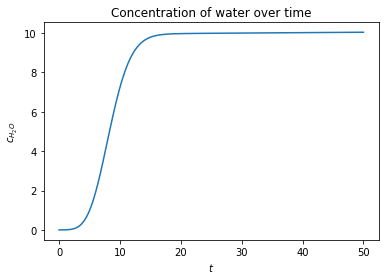
\includegraphics[width=\textwidth]{water.png}
% \caption{Image on the left}\label{subfig:left}
% \end{subfigure}
% \begin{subfigure}[b]{.4\textwidth}
% 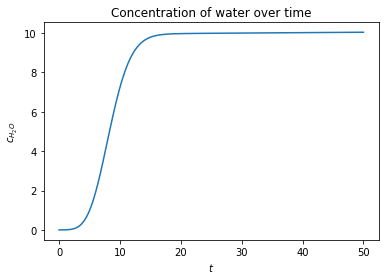
\includegraphics[width=\textwidth]{water.png}
% \caption{Image on the right}\label{subfig:right}
% \end{subfigure}
% \caption{Two images}\label{fig:subfigures}
% \end{figure}

% \section{Strengths and Weaknesses}
% \subsection{Strengths}
% \begin{itemize}
%     \item First one...
%     \item Second one ...
% \end{itemize}

% \subsection{Weaknesses}
% \begin{itemize}
%     \item Only one ...
%  \end{itemize}



% 参考文献,此处以 GB 引用格式为例
\begin{thebibliography}{99}
\addtolength{\itemsep}{-0.5 em} % 缩小参考文献间的垂直间距
\setlength{\itemsep}{-5pt}
\bibitem{1} Swain R B, Ranganathan S. Modeling interlinkages between sustainable development goals using network analysis[J]. World Development, 2021, 138: 105136.
\bibitem{2} Dalampira E S, Nastis S A. Mapping sustainable development goals: A network analysis framework[J]. Sustainable Development, 2020, 28(1): 46-55.
\bibitem{3} Le Blanc D. Towards integration at last? The sustainable development goals as a network of targets[J]. Sustainable Development, 2015, 23(3): 176-187.
\bibitem{4} Easterly W. The trouble with the sustainable development goals[J]. Current History, 2015, 114(775): 322.
\bibitem{5} Wang Y, Lu Y, He G, et al. Spatial variability of sustainable development goals in China: A provincial level evaluation[J]. Environmental Development, 2020, 35: 100483.
\bibitem{6} A mathematical modeling approach from nonlinear dynamics to complex systems[M]. Springer, 2018.
\bibitem{7} Liengpunsakul S. Artificial intelligence and sustainable development in China[J]. The Chinese Economy, 2021, 54(4): 235-248.
\bibitem{8} Weitz N, Carlsen H, Nilsson M, et al. Towards systemic and contextual priority setting for implementing the 2030 Agenda[J]. Sustainability science, 2018, 13: 531-548.
\bibitem{9} Allen C, Metternicht G, Wiedmann T. Prioritising SDG targets: Assessing baselines, gaps and interlinkages[J]. Sustainability Science, 2019, 14: 421-438.
\bibitem{10} Clemente-Suárez V J, Rodriguez-Besteiro S, Cabello-Eras J J, et al. Sustainable development goals in the COVID-19 pandemic: A narrative review[J]. Sustainability, 2022, 14(13): 7726.
\bibitem{11} Nilsson M, Griggs D, Visbeck M. Policy: map the interactions between Sustainable Development Goals[J]. Nature, 2016, 534(7607): 320-322.
\bibitem{12} Weitz N, Persson Å, Nilsson M, et al. Sustainable development goals for Sweden: insights on setting a national agenda[M]. Stockholm Environment Institute., 2015.
\end{thebibliography}

% % 以下为附录内容
% % 如您的论文中不需要附录,请自行删除
% \begin{subappendices}  % 附录环境

% \section{Appendix A: Further on \LaTeX}
% To clarify the importance of using \LaTeX\ in MCM or ICM, several points need to be covered, which are \ldots

% To be more specific, \ldots

% All in all, \ldots

% Anyway, nobody \textbf{really} needs such appendix \ldots

% \section{Appendix B: Program Codes}
% Here are the program codes we used in our research.

% % 代码环境示例三则
% % 如您的论文不需要展示代码,请删除
% % 更多用法,请参考 listings 宏包文档

% % Python 代码示例
% \begin{lstlisting}[language=Python, name={test.py}]
% # Python code example
% for i in range(10):
%     print('Hello, world!')
% \end{lstlisting}

% % MATLAB 代码示例
% \begin{lstlisting}[language=MATLAB, name={test.m}]
% % MATLAB code example
% for i = 1:10
%     disp("hello, world!");
% end
% \end{lstlisting}

% % C++ 代码示例
% \begin{lstlisting}[language=C++, name={test.cpp}]
% // C++ code example
% #include <iostream>
% using namespace std;

% int main() {
%     for (int i = 0; i < 10; i++)
%         cout << "hello, world" << endl;
%     return 0;
% }
% \end{lstlisting}

% \end{subappendices}  % 附录内容结束

\end{document}  % 结束
